\documentclass[preprint,12pt]{elsarticle}
% RESS (Reliability Engineering & System Safety) review version. All numbers come from numbers.tex and
% ../proofs_numbers.tex (generated from results/*.json); tables from tools/make_main_tables.py; bibliography refs_ress.bib
% (tools/make_bib.py, DOIs checked on Crossref). Build: bash build.sh main_ress
\usepackage{lineno}
\usepackage{amsmath,amssymb,amsthm}
\usepackage{graphicx}
\usepackage{booktabs}
\usepackage{array}
\usepackage{tikz}
\usetikzlibrary{arrows.meta,positioning}
\usepackage{xurl}
\usepackage[hidelinks]{hyperref}
\newcolumntype{L}[1]{>{\raggedright\arraybackslash}p{#1}}
% generated by tools/make_numbers.py from results/*.json -- DO NOT EDIT BY HAND (checklist C6)
\newcommand{\nNzero}{59} % n0(5%,5%) = ceil(ln .05/ln .95); c2_mc.primary n0
\newcommand{\nNzeroTwenty}{14} % n0(20%,5%); exchange_rate_v2.marked.OP*.n0
\newcommand{\ncExactA}{8} % c2_mc.primary[delta'=0.075].c_integer_exact (events)
\newcommand{\ncStarA}{7} % c2_mc.primary[delta'=0.075].c_star (continuous lower bound)
\newcommand{\ncSaveA}{14\%} % c / n0 = 8/59
\newcommand{\ncExactB}{14} % c2_mc.primary[delta'=0.1].c_integer_exact (events)
\newcommand{\ncStarB}{13} % c2_mc.primary[delta'=0.1].c_star (continuous lower bound)
\newcommand{\ncSaveB}{24\%} % c / n0 = 14/59
\newcommand{\ncExactC}{22} % c2_mc.primary[delta'=0.15].c_integer_exact (events)
\newcommand{\ncStarC}{21} % c2_mc.primary[delta'=0.15].c_star (continuous lower bound)
\newcommand{\ncSaveC}{37\%} % c / n0 = 22/59
\newcommand{\ncExactD}{27} % c2_mc.primary[delta'=0.2].c_integer_exact (events)
\newcommand{\ncStarD}{27} % c2_mc.primary[delta'=0.2].c_star (continuous lower bound)
\newcommand{\ncSaveD}{46\%} % c / n0 = 27/59
\newcommand{\nCtwoNgrid}{40} % c2_mc grid points
\newcommand{\nCtwoMaxDevPP}{0.29} % c2_mc.max_abs_dev_pp_exact (percentage points, 40-point grid, MC 1e5)
\newcommand{\nCthreeA}{72} % c3_numbers q_U=0
\newcommand{\nCthreeB}{91} % q_U=1%
\newcommand{\nCthreeC}{122} % q_U=2%
\newcommand{\nPopScenesTen}{29} % c4_power.scenes_needed_c4a_pop U<=10% (J=0)
\newcommand{\nPopScenesFive}{59} % U<=5% (J=0)
\newcommand{\nLemmaMin}{0.2500} % c4_power.lemma_mean_median.min_F_floor_Np
\newcommand{\nCorpusT}{3,170} % corpus17_manifest.counts.mode_T_total (events)
\newcommand{\nCorpusTvideos}{101} % mode_T_real_videos
\newcommand{\nMainScenes}{48} % calibration_scenes.main
\newcommand{\nNightScenes}{6} % calibration_scenes.night
\newcommand{\nTurbScenes}{4} % calibration_scenes.turbulence
\newcommand{\nPTZScenes}{4} % calibration_scenes.excluded_PTZ
\newcommand{\nJitterScenes}{26} % calibration_scenes.jitter (cameraJitter, post-F1 correction v1.1)
\newcommand{\nMainCDnet}{28} % p1_background17.by_tier.main CDnet
\newcommand{\nMainLASIESTA}{20} % by_tier.main LASIESTA
\newcommand{\nMainN}{114} % e0_units main N (events, d>=32)
\newcommand{\nMainDw}{0} % e0_units main D_worst_phase.num (events)
\newcommand{\nMainDwPct}{0.00\%} % 0/114
\newcommand{\nMainDexp}{0.0000} % expected discordant events (mean over phases and 3 variants)
\newcommand{\nMainDexpPct}{0.00\%} % 0.0000/114
\newcommand{\nMainUfleet}{2.59\%} % U_CP(0,114)
\newcommand{\nMainJ}{0} % scenes with a discordant event
\newcommand{\nMainM}{48} % scenes
\newcommand{\nMainUpop}{6.05\%} % U_CP(0,48)
\newcommand{\nNightN}{25} % night events d>=32
\newcommand{\nNightDw}{12} % night worst-phase discordant
\newcommand{\nNightDwPct}{48\%} % 12/25
\newcommand{\nNightDexp}{8.21} % night expected discordant events (mean over phases and 3 variants)
\newcommand{\nNightDexpMaj}{8.31} % night expected discordant events, majority rule
\newcommand{\nNightUfleet}{65.9\%} % night U_fleet worst
\newcommand{\nNightJ}{5} % night J
\newcommand{\nNightUpop}{99.1\%} % night U_pop
\newcommand{\nJitN}{62} % jitter events d>=32
\newcommand{\nJitDw}{3} % jitter worst-phase discordant
\newcommand{\nJitUfleet}{12.0\%} % jitter U_fleet worst
\newcommand{\nJitJ}{1} % jitter J
\newcommand{\nJitM}{26} % jitter scenes
\newcommand{\nJitUpop}{17.0\%} % jitter U_pop
\newcommand{\nJitFC}{0} % jitter cameras falsely certified, main-only calibration, phase-averaged (OP*)
\newcommand{\nJitFCch}{0} % same at (16,16)
\newcommand{\nJitPgt}{0} % jitter cameras with phase-averaged p_s > eps (OP*)
\newcommand{\nTurbN}{2} % turbulence events d>=32 (scenes run: 2)
\newcommand{\nAllN}{203} % all tiers N
\newcommand{\nAllDw}{16} % all tiers worst-phase discordant
\newcommand{\nAllUfleet}{11.7\%} % all tiers U_fleet
\newcommand{\nAllJ}{7} % all tiers J
\newcommand{\nAllM}{82} % all tiers scenes
\newcommand{\nAllUpop}{15.4\%} % all tiers U_pop
\newcommand{\nPmainOP}{0.88\%} % 1.0000/114 (phase-expected)
\newcommand{\nPmainOPshort}{0.9\%} % same, 1 decimal (abstract)
\newcommand{\nRealMissExpOP}{1.00} % expected real-miss events at OP* (main)
\newcommand{\nRealMissEvOP}{1} % events with a real miss at >= 1 phase
\newcommand{\nRealMissScOP}{1} % scenes with a real miss
\newcommand{\nRecallOP}{100\%} % 1.00/1.00
\newcommand{\nRecallNight}{8\%} % 0.75/9.06
\newcommand{\nChRealMissEv}{13} % (16,16) real-miss events
\newcommand{\nChTwinAlso}{13} % (16,16) twin also misses
\newcommand{\nChRecall}{88\%} % (16,16) recall expected
\newcommand{\nChN}{129} % (16,16) events
\newcommand{\nOldPhat}{11.3\%} % operating_points_v2.final_operating_point.p_hat over 161 CDnet events (all tiers)
\newcommand{\nOldN}{161} % events behind the pooled 11.3%
\newcommand{\nOldNreq}{112} % direct n at 11.3%
\newcommand{\nLosoOP}{0} % LOSO violations D_s > U_pop(-s), OP* (of 48)
\newcommand{\nLosoCh}{0} % LOSO violations, (16,16) (of 48)
\newcommand{\nLosoOPFC}{0} % OP* LOSO false certificates
\newcommand{\nLosoChFC}{0} % (16,16) LOSO false certificates
\newcommand{\nChUpop}{12.5\%} % U_CP(2,48)
\newcommand{\nChJ}{2} % (16,16) J
\newcommand{\nMcFC}{0.0\%} % MC 10,000 false-cert rate OP*
\newcommand{\nScenesPgtEpsOP}{1} % static scenes with p_s > eps at OP* (validity_audit loso.scenes_p_gt_eps)
\newcommand{\nMcFCch}{0.0\%} % MC false-cert rate (16,16)
\newcommand{\nMustFailScenes}{3} % K=48 scenes with p_s > eps
\newcommand{\nMustFailRefuse}{100\%} % refusal rate
\newcommand{\nMustFailApp}{1} % scenes with detector-miss p > eps
\newcommand{\nFleetMeasPB}{0.0272} % max exact PB failure over 12 cases
\newcommand{\nFleetMeasCases}{12} % cases
\newcommand{\nPopTightMax}{0.041} % C4a-pop tight-case max failure (MC 1e5)
\newcommand{\nLeakUpopZero}{6.1\%} % k=0 U_pop OP*
\newcommand{\nLeakUpopSix}{18.5\%} % k=6 U_pop OP*
\newcommand{\nLeakUpopZeroCh}{12.5\%} % k=0 U_pop (16,16)
\newcommand{\nLeakUpopSixCh}{23.0\%} % k=6 (16,16)
\newcommand{\nLeakWithdrawK}{3} % smallest k with all subsets withdrawn (U > eps/2), OP*
\newcommand{\nLeakWithdrawKfirst}{2} % smallest k with some subsets withdrawn, OP*
\newcommand{\nNightFC}{4} % night cameras falsely certified, judged alone (OP*)
\newcommand{\nNightFCch}{3} % same at (16,16)
\newcommand{\nNightPgt}{4} % night cameras with p_s > eps
\newcommand{\nMainFCleak}{0} % main cameras falsely certified, any k
\newcommand{\nSavedOP}{14} % median real events saved per camera, OP*, q known
\newcommand{\nSavedCamOP}{46} % cameras saving (of 48)
\newcommand{\nSavedFinCamOP}{3} % cameras saving with the twin as built
\newcommand{\nSavedFinOP}{0} % median saved, twin as built
\newcommand{\nTwinRunsOP}{28} % exchange_rate.marked.OP*.q_known.n_twin_events_needed_median
\newcommand{\nCpuPerSavedOP}{0.069} % CPU-hours per saved real event, OP* median
\newcommand{\nBreakEven}{14} % 1/c: events/hour (assumes 1 CPU-hour = 1 hour of waiting)
\newcommand{\nSavedCh}{30} % (16,16) saved per camera
\newcommand{\nSavedOPC}{46} % OP-C saved per camera
\newcommand{\nTwinCostScene}{0.20} % CPU-hours per scene, median (C0 build)
\newcommand{\nTwinCostTotal}{14.1} % CPU-hours, 48 main-domain scenes
\newcommand{\nGridPts}{70} % grid points eps=20%
\newcommand{\nGridFinMax}{4} % max cameras saving with the twin as built, any grid point
\newcommand{\nCtwoTwinPass}{73.3\%} % twin pass probability (MC 1e5)
\newcommand{\nCtwoTwinPassShort}{73\%} % twin pass probability, rounded: share of the exact credit realised on average
\newcommand{\nCtwoFCA}{6.7\%} % false cert at p=eps, delta'=0.075
\newcommand{\nCtwoFCB}{8.4\%} % false cert at p=eps, delta'=0.1
\newcommand{\nCtwoFCC}{12.2\%} % false cert at p=eps, delta'=0.15
\newcommand{\nCtwoFCD}{15.6\%} % false cert at p=eps, delta'=0.2
\newcommand{\nCtwoBMCPass}{0\%} % BMC-synth pass probability
\newcommand{\nCtwoBMCN}{30} % BMC-synth events d>=32
\newcommand{\nIWtemporal}{0.64} % iw_ablation_v2 all targets, logistic, temporal
\newcommand{\nIWgeometry}{0.94} % all targets, geometry
\newcommand{\nIWappearance}{0.77} % all targets, appearance only
\newcommand{\nIWtemporalCD}{0.61} % CDnet targets (supplement)
\newcommand{\nIWgeometryCD}{0.96} % CDnet targets
\newcommand{\nIWappearanceCD}{0.75} % CDnet targets
\newcommand{\nClampShare}{70\%} % share of twin frames with a width clamp
\newcommand{\nClampExtraDrop}{3.0} % extra twin hit-rate drop (points) on clamped frames
\newcommand{\nClampPairs}{631} % event x variant pairs
\newcommand{\nCfiveQzero}{1.37\%} % q at x=0
\newcommand{\nCfiveQfifty}{2.36\%} % q at x=50%
\newcommand{\nConfTwin}{0.78} % median detector confidence on twin hits
\newcommand{\nConfReal}{0.87} % median detector confidence on real hits
\newcommand{\nOrigN}{116} % original definition events at OP*
\newcommand{\nOrigJ}{0} % original definition J
\newcommand{\nPmainOPA}{0.88\%} % OP-A main p-hat
\newcommand{\nDexpOPA}{0.00} % OP-A expected discordant events
\newcommand{\nPmainOPC}{0.88\%} % OP-C main p-hat
\newcommand{\nDexpOPC}{0.00} % OP-C expected discordant events
\newcommand{\nTurbDw}{1} % turbulence worst-phase discordant events
\newcommand{\nTurbUfleet}{97.5\%} % turbulence U_fleet
\newcommand{\nTurbJ}{1} % turbulence J
\newcommand{\nTurbM}{2} % turbulence scenes run
\newcommand{\nTurbUpop}{97.5\%} % turbulence U_pop
\newcommand{\nUpopJzero}{6.1\%} % U_CP(0,48), formula (worked example)
\newcommand{\nUpopJone}{9.5\%} % U_CP(1,48), formula (worked example)
\newcommand{\nUpopJtwo}{12.5\%} % U_CP(2,48), formula (worked example)
\newcommand{\nUpopJthree}{15.4\%} % U_CP(3,48), formula (worked example)
\newcommand{\nPiStarA}{6.1\%} % Result 2 threshold pi* on the simulator pass probability, delta'=0.075, eps=delta=5%
\newcommand{\nPiStarB}{3.0\%} % Result 2 threshold pi* on the simulator pass probability, delta'=0.1, eps=delta=5%
\newcommand{\nPiStarC}{1.5\%} % Result 2 threshold pi* on the simulator pass probability, delta'=0.15, eps=delta=5%
\newcommand{\nPiStarD}{1.0\%} % Result 2 threshold pi* on the simulator pass probability, delta'=0.2, eps=delta=5%
\newcommand{\nPAccept}{95.8\%} % share of static cameras accepted by the twin route at OP* (cameras saving / 48)
\newcommand{\nAcceptInflation}{0.3} % U_delta/2(J,48) (1/P(accept) - 1), percentage points
\newcommand{\nUhalfJzero}{7.4\%} % U_CP(0,48) at delta/2 (decision level)
\newcommand{\nUhalfJone}{11.1\%} % U_CP(1,48) at delta/2 (decision level)
\newcommand{\nUhalfJtwo}{14.3\%} % U_CP(2,48) at delta/2 (decision level)
\newcommand{\nUhalfJthree}{17.2\%} % U_CP(3,48) at delta/2 (decision level)
\newcommand{\nPopScenesQuarter}{119} % eps=5%: smallest m with U_CP(0,m) <= eps/2 = 2.5% (J=0, delta=5%)
\newcommand{\nMCScenes}{4} % calibration_scenes.excluded_MC (LASIESTA moving camera)
\newcommand{\nCalibPerCam}{2.4} % annotated calibration events at OP* per static camera (N/m)
\newcommand{\nDirectPooledU}{4.1\%} % direct CP on the calibrated cameras' real misses (events missed at some phase / N)
\newcommand{\nCtwoCFA}{6.7\%} % closed form P(pass)(1-eps)^n1+(1-P(pass))(1-eps)^n0, delta'=0.075
\newcommand{\nCtwoCFB}{8.6\%} % closed form P(pass)(1-eps)^n1+(1-P(pass))(1-eps)^n0, delta'=0.1
\newcommand{\nCtwoCFC}{12.3\%} % closed form P(pass)(1-eps)^n1+(1-P(pass))(1-eps)^n0, delta'=0.15
\newcommand{\nCtwoCFD}{15.5\%} % closed form P(pass)(1-eps)^n1+(1-P(pass))(1-eps)^n0, delta'=0.2
\newcommand{\nCtwoSE}{0.1\%} % MC standard error bound sqrt(0.1*0.9/1e5)=0.09 pts, rounded to 0.1
\newcommand{\nNightHeldD}{23.2\%} % night held-out median per-scene D (pre-registered criterion <= 5%)
\newcommand{\nNightHeldN}{14} % night held-out events at OP*
\newcommand{\nNightBaseD}{47.2\%} % night tuning scenes, base twin, D-hat (phase-averaged)
\newcommand{\nNightProfD}{47.0\%} % night tuning scenes, kept profile, D-hat
\newcommand{\nDefAllA}{161} % primary definition, events of all durations (static)
\newcommand{\nDefAllO}{222} % original definition, events of all durations (static)
\newcommand{\nOrigChJ}{3} % original definition (16,16) J
\newcommand{\nOrigChUpop}{15.4\%} % original (16,16) U_pop
\newcommand{\nOrigOPUfleet}{2.55\%} % original OP* U_fleet (worst phase)
\newcommand{\nOrigOPDw}{0} % original OP* disc
\newcommand{\nTpOPS}{0.88\%} % OP* static-domain p-hat
\newcommand{\nTndOPS}{14} % OP* n_direct (80% power at p-hat)
\newcommand{\nTsvOPS}{14} % OP* saved per camera (median)
\newcommand{\nTcamOPS}{46} % OP* cameras saving (of 48)
\newcommand{\nTcamfinOPS}{3} % OP* cameras saving, twin as built
\newcommand{\nTrunsOPS}{28} % OP* twin runs needed per camera
\newcommand{\nTcpuOPS}{0.069} % OP* CPU-h per saved event
\newcommand{\nTpOPA}{0.88\%} % OP-A static-domain p-hat
\newcommand{\nTndOPA}{14} % OP-A n_direct (80% power at p-hat)
\newcommand{\nTsvOPA}{14} % OP-A saved per camera (median)
\newcommand{\nTcamOPA}{47} % OP-A cameras saving (of 48)
\newcommand{\nTcamfinOPA}{3} % OP-A cameras saving, twin as built
\newcommand{\nTrunsOPA}{28} % OP-A twin runs needed per camera
\newcommand{\nTcpuOPA}{0.064} % OP-A CPU-h per saved event
\newcommand{\nTpOPC}{0.88\%} % OP-C static-domain p-hat
\newcommand{\nTndOPC}{46} % OP-C n_direct (80% power at p-hat)
\newcommand{\nTsvOPC}{46} % OP-C saved per camera (median)
\newcommand{\nTcamOPC}{47} % OP-C cameras saving (of 48)
\newcommand{\nTcamfinOPC}{0} % OP-C cameras saving, twin as built
\newcommand{\nTrunsOPC}{149} % OP-C twin runs needed per camera
\newcommand{\nTcpuOPC}{0.104} % OP-C CPU-h per saved event
\newcommand{\nTpCH}{4.26\%} % challenge_16_16 static-domain p-hat
\newcommand{\nTndCH}{30} % challenge_16_16 n_direct (80% power at p-hat)
\newcommand{\nTsvCH}{30} % challenge_16_16 saved per camera (median)
\newcommand{\nTcamCH}{45} % challenge_16_16 cameras saving (of 48)
\newcommand{\nTcamfinCH}{0} % challenge_16_16 cameras saving, twin as built
\newcommand{\nTrunsCH}{66} % challenge_16_16 twin runs needed per camera
\newcommand{\nTcpuCH}{0.078} % challenge_16_16 CPU-h per saved event
\newcommand{\nWPSpMain}{0.9\%} % worst-phase real miss rate, main, OP* (events missed at >= 1 phase / N=114)
\newcommand{\nWPSqMain}{3.5\%} % worst-phase twin miss rate (majority), main, OP*
\newcommand{\nPASpMain}{0.9\%} % phase-averaged real miss rate, main, OP*
\newcommand{\nPASqMain}{1.4\%} % phase-averaged twin miss rate (majority), main, OP*
\newcommand{\nWPSpJit}{4.8\%} % worst-phase real miss rate, jitter, OP* (events missed at >= 1 phase / N=62)
\newcommand{\nWPSqJit}{0.0\%} % worst-phase twin miss rate (majority), jitter, OP*
\newcommand{\nPASpJit}{0.5\%} % phase-averaged real miss rate, jitter, OP*
\newcommand{\nPASqJit}{0.0\%} % phase-averaged twin miss rate (majority), jitter, OP*
\newcommand{\nWPSpNight}{52.0\%} % worst-phase real miss rate, night, OP* (events missed at >= 1 phase / N=25)
\newcommand{\nWPSqNight}{16.0\%} % worst-phase twin miss rate (majority), night, OP*
\newcommand{\nPASpNight}{36.2\%} % phase-averaged real miss rate, night, OP*
\newcommand{\nPASqNight}{4.8\%} % phase-averaged twin miss rate (majority), night, OP*
\newcommand{\nWPSpTurb}{50.0\%} % worst-phase real miss rate, turbulence, OP* (events missed at >= 1 phase / N=2)
\newcommand{\nWPSqTurb}{0.0\%} % worst-phase twin miss rate (majority), turbulence, OP*
\newcommand{\nPASpTurb}{6.2\%} % phase-averaged real miss rate, turbulence, OP*
\newcommand{\nPASqTurb}{0.0\%} % phase-averaged twin miss rate (majority), turbulence, OP*
\newcommand{\nWPSpAll}{8.9\%} % worst-phase real miss rate, all_tiers, OP* (events missed at >= 1 phase / N=203)
\newcommand{\nWPSqAll}{3.9\%} % worst-phase twin miss rate (majority), all_tiers, OP*
\newcommand{\nPASpAll}{5.2\%} % phase-averaged real miss rate, all_tiers, OP*
\newcommand{\nPASqAll}{1.4\%} % phase-averaged twin miss rate (majority), all_tiers, OP*
\newcommand{\nWXSp}{0.9\%} % pooled worst-phase real miss rate, main, OP*
\newcommand{\nWXSnd}{14} % direct plan at the worst-phase p, OP*
\newcommand{\nWXSacc}{44} % cameras accepted with worst-phase q (of 48), OP*
\newcommand{\nWXSsaved}{14} % median real events saved per camera, worst-phase, OP*
\newcommand{\nWXSfa}{0} % accepted cameras with worst-phase p_s > eps, OP*
\newcommand{\nWXSruns}{28} % twin runs needed per camera (median), worst-phase q, OP*
\newcommand{\nWPSDwMain}{0} % worst-phase discordant events, main, OP* (of N=114)
\newcommand{\nWPSNMain}{114} % main events, OP*
\newcommand{\nWPSUfMain}{2.6\%} % U_CP(0,114), main, OP*
\newcommand{\nWPSJMain}{0} % main scenes with a worst-phase discordant event, OP* (of 48)
\newcommand{\nWPSUpMain}{6.1\%} % U_CP(0,48), main, OP*
\newcommand{\nWPSNJit}{62} % jitter events, OP*
\newcommand{\nWPSDwJit}{3} % jitter worst-phase discordant events, OP*
\newcommand{\nOODSJitcams}{26} % jitter cameras judged with a main-only calibration, OP*
\newcommand{\nOODSJitacc}{26} % jitter cameras accepted (worst-phase q_w + U_delta/2(J_main,m_main) <= eps), OP*
\newcommand{\nOODSJitfa}{1} % jitter cameras falsely accepted (accepted and p_w > eps), OP*
\newcommand{\nOODSJitpgt}{1} % jitter cameras with p_w > eps, OP*
\newcommand{\nOODSNightcams}{6} % night cameras judged with a main-only calibration, OP*
\newcommand{\nOODSNightacc}{5} % night cameras accepted (worst-phase q_w + U_delta/2(J_main,m_main) <= eps), OP*
\newcommand{\nOODSNightfa}{4} % night cameras falsely accepted (accepted and p_w > eps), OP*
\newcommand{\nOODSNightpgt}{5} % night cameras with p_w > eps, OP*
\newcommand{\nOODSJitFApw}{37.5\%} % p_w of the falsely accepted jitter camera traffic, OP*
\newcommand{\nWPCpMain}{10.1\%} % worst-phase real miss rate, main, challenge_16_16 (events missed at >= 1 phase / N=129)
\newcommand{\nWPCqMain}{13.2\%} % worst-phase twin miss rate (majority), main, challenge_16_16
\newcommand{\nPACpMain}{4.3\%} % phase-averaged real miss rate, main, challenge_16_16
\newcommand{\nPACqMain}{6.5\%} % phase-averaged twin miss rate (majority), main, challenge_16_16
\newcommand{\nWPCpJit}{10.4\%} % worst-phase real miss rate, jitter, challenge_16_16 (events missed at >= 1 phase / N=67)
\newcommand{\nWPCqJit}{0.0\%} % worst-phase twin miss rate (majority), jitter, challenge_16_16
\newcommand{\nPACpJit}{1.9\%} % phase-averaged real miss rate, jitter, challenge_16_16
\newcommand{\nPACqJit}{0.0\%} % phase-averaged twin miss rate (majority), jitter, challenge_16_16
\newcommand{\nWPCpNight}{63.9\%} % worst-phase real miss rate, night, challenge_16_16 (events missed at >= 1 phase / N=36)
\newcommand{\nWPCqNight}{30.6\%} % worst-phase twin miss rate (majority), night, challenge_16_16
\newcommand{\nPACpNight}{49.7\%} % phase-averaged real miss rate, night, challenge_16_16
\newcommand{\nPACqNight}{8.0\%} % phase-averaged twin miss rate (majority), night, challenge_16_16
\newcommand{\nWPCpTurb}{50.0\%} % worst-phase real miss rate, turbulence, challenge_16_16 (events missed at >= 1 phase / N=2)
\newcommand{\nWPCqTurb}{0.0\%} % worst-phase twin miss rate (majority), turbulence, challenge_16_16
\newcommand{\nPACpTurb}{6.2\%} % phase-averaged real miss rate, turbulence, challenge_16_16
\newcommand{\nPACqTurb}{0.0\%} % phase-averaged twin miss rate (majority), turbulence, challenge_16_16
\newcommand{\nWPCpAll}{18.8\%} % worst-phase real miss rate, all_tiers, challenge_16_16 (events missed at >= 1 phase / N=234)
\newcommand{\nWPCqAll}{12.0\%} % worst-phase twin miss rate (majority), all_tiers, challenge_16_16
\newcommand{\nPACpAll}{10.6\%} % phase-averaged real miss rate, all_tiers, challenge_16_16
\newcommand{\nPACqAll}{4.8\%} % phase-averaged twin miss rate (majority), all_tiers, challenge_16_16
\newcommand{\nWXCp}{10.1\%} % pooled worst-phase real miss rate, main, challenge_16_16
\newcommand{\nWXCnd}{88} % direct plan at the worst-phase p, challenge_16_16
\newcommand{\nWXCacc}{43} % cameras accepted with worst-phase q (of 48), challenge_16_16
\newcommand{\nWXCsaved}{88} % median real events saved per camera, worst-phase, challenge_16_16
\newcommand{\nWXCfa}{0} % accepted cameras with worst-phase p_s > eps, challenge_16_16
\newcommand{\nWXCruns}{66} % twin runs needed per camera (median), worst-phase q, challenge_16_16
\newcommand{\nWPCDwMain}{5} % worst-phase discordant events, main, challenge_16_16 (of N=129)
\newcommand{\nWPCNMain}{129} % main events, challenge_16_16
\newcommand{\nWPCUfMain}{8.0\%} % U_CP(5,129), main, challenge_16_16
\newcommand{\nWPCJMain}{2} % main scenes with a worst-phase discordant event, challenge_16_16 (of 48)
\newcommand{\nWPCUpMain}{12.5\%} % U_CP(2,48), main, challenge_16_16
\newcommand{\nWPCNJit}{67} % jitter events, challenge_16_16
\newcommand{\nWPCDwJit}{7} % jitter worst-phase discordant events, challenge_16_16
\newcommand{\nOODCJitcams}{26} % jitter cameras judged with a main-only calibration, challenge_16_16
\newcommand{\nOODCJitacc}{26} % jitter cameras accepted (worst-phase q_w + U_delta/2(J_main,m_main) <= eps), challenge_16_16
\newcommand{\nOODCJitfa}{1} % jitter cameras falsely accepted (accepted and p_w > eps), challenge_16_16
\newcommand{\nOODCJitpgt}{1} % jitter cameras with p_w > eps, challenge_16_16
\newcommand{\nOODCNightcams}{6} % night cameras judged with a main-only calibration, challenge_16_16
\newcommand{\nOODCNightacc}{3} % night cameras accepted (worst-phase q_w + U_delta/2(J_main,m_main) <= eps), challenge_16_16
\newcommand{\nOODCNightfa}{3} % night cameras falsely accepted (accepted and p_w > eps), challenge_16_16
\newcommand{\nOODCNightpgt}{6} % night cameras with p_w > eps, challenge_16_16
\newcommand{\nOODCJitFApw}{53.8\%} % p_w of the falsely accepted jitter camera traffic, challenge_16_16
\newcommand{\nSiteSm}{17} % sites (CDnet categories + LASIESTA groups), OP*
\newcommand{\nSiteSJ}{0} % sites with a discordant event, OP*
\newcommand{\nSiteSU}{16.2\%} % site-level population bound U_CP(J_site, m_site), OP*
\newcommand{\nSiteSloso}{0} % leave-one-site-out violations, OP*
\newcommand{\nSiteCm}{17} % sites (CDnet categories + LASIESTA groups), challenge_16_16
\newcommand{\nSiteCJ}{1} % sites with a discordant event, challenge_16_16
\newcommand{\nSiteCU}{25.0\%} % site-level population bound U_CP(J_site, m_site), challenge_16_16
\newcommand{\nSiteCloso}{1} % leave-one-site-out violations, challenge_16_16
\newcommand{\nRepoTag}{ress-v1.2} % artifact release tag
\newcommand{\nRepoHashShort}{890465bd9267} % commit A (tagged) short hash

\providecommand{\nRepoHashShort}{(hash set at tagging)}
\newcommand{\repohash}{\nRepoHashShort}
% generated by tools/make_proofs_numbers.py from results/*.json -- do not edit
\newcommand{\numConeClosed}{0.0485}
\newcommand{\numConeMC}{0.0491}
\newcommand{\numCtwoMaxDev}{0.29}
\newcommand{\numCtwoNgrid}{40}
\newcommand{\numCtwoAllMax}{yes}
\newcommand{\numCtwoTwinPass}{98.2\%}
\newcommand{\numCtwoFCA}{7.2\%}
\newcommand{\numCtwoCredA}{7.9}
\newcommand{\numCtwoFCB}{10.1\%}
\newcommand{\numCtwoCredB}{13.7}
\newcommand{\numCtwoFCC}{14.8\%}
\newcommand{\numCtwoCredC}{21.6}
\newcommand{\numCtwoFCD}{19.3\%}
\newcommand{\numCtwoCredD}{26.5}
\newcommand{\numCtwoBMCPass}{0.0\%}
\newcommand{\numCthreeA}{72}
\newcommand{\numCthreeB}{91}
\newcommand{\numCthreeC}{122}
\newcommand{\numLemmaMin}{0.2500}
\newcommand{\numFleetPBmax}{0.0471}
\newcommand{\numFleetMCmax}{0.0473}
\newcommand{\numFleetNpat}{6}
\newcommand{\numFleetMeasPBmax}{0.0126}
\newcommand{\numFleetMeasMCmax}{0.0129}
\newcommand{\numFleetMeasN}{15}
\newcommand{\numPopFailMax}{0.0401}
\newcommand{\numCfourbFailMax}{0.0286}
\newcommand{\numPopScenesTen}{29}
\newcommand{\numPopScenesFive}{59}
\newcommand{\numLosoViolNum}{2}
\newcommand{\numLosoViolDen}{78}
\newcommand{\numCfiveAll}{yes}
\newcommand{\numCfiveQzero}{0.87\%}
\newcommand{\numCfiveQfifty}{1.67\%}

\hypersetup{pdftitle={No Free Credit: How Much Simulated Evidence Can Replace Real Events in Zero-Failure Reliability
Demonstration of Perception Systems}, pdfauthor={Lam Quoc Dat},
pdfkeywords={reliability demonstration, zero-failure testing, synthetic data, digital twin, success-run, perception system,
transfer bound}}

\newtheorem{theorem}{Theorem}[section]
\newtheorem{proposition}[theorem]{Proposition}
\newtheorem{lemma}[theorem]{Lemma}
\newtheorem{corollary}[theorem]{Corollary}
\theoremstyle{definition}
\newtheorem{definition}[theorem]{Definition}
\theoremstyle{remark}
\newtheorem{remark}[theorem]{Remark}
\newcommand{\PP}{\mathbb{P}}
\newcommand{\EE}{\mathbb{E}}
\newcommand{\UCP}{U}
\newcommand{\Bin}{\mathrm{Bin}}
\newcommand{\Bern}{\mathrm{Bern}}
\newcommand{\OPs}{$\mathrm{OP}^\ast$}
\newcommand{\paperstart}[2]{#1#2}
\emergencystretch=2em

\journal{Reliability Engineering \& System Safety}

\begin{document}
\begin{frontmatter}
\title{No Free Credit: How Much Simulated Evidence Can Replace Real Events in Zero-Failure Reliability Demonstration of
Perception Systems}
\author{Lam Quoc Dat\fnref{orcid}}
\ead{lamquocdat@gmail.com}
\fntext[orcid]{ORCID: \href{https://orcid.org/0009-0004-5432-9343}{0009-0004-5432-9343}}
\affiliation{organization={School of Business and Technology (FSB), FPT University},
  city={Ho Chi Minh City}, country={Vietnam}}

\begin{abstract}
% RESS abstract (<= 200 words; checked by tools/check_front_ress.py). Numbers via numbers.tex.
A perception system on a new fixed camera is often accepted by a zero-failure reliability demonstration: a fixed number
of real events, the zero-failure sample size (\nNzero{} events for 95\% confidence that at most 5\% of events are
missed), must pass without a miss. How many can simulated evidence replace? We prove that,
without an assumption linking the simulator to reality, independent simulated data cannot shorten the demonstration;
that accepting a larger error probability buys an exactly computable number of events; and that a synthetic twin paired
with each real event bounds the real miss rate by the twin miss rate plus a discordance rate, which pays off only
through a transfer bound priced in calibration scenes. On \nMainScenes{} fixed-camera scenes, real misses are rare at the pre-specified operating point (\nPmainOPshort), so
it is untested there. If calibration carries over, a twin run about \nTwinRunsOP{} times per camera would save at most \nSavedOP{} events per camera at a 20\% target; the twin as built saves none. The transfer certificate stands at scene level but is withdrawn at site level (\nSiteSm{} sites). Two named failure modes: night and
camera-jitter cameras pass through (\nOODSNightfa{} of \nOODSNightcams{} and \nOODSJitfa{} of \nOODSJitcams{} falsely accepted).

\end{abstract}

\begin{keyword}
reliability demonstration \sep zero-failure testing \sep synthetic data \sep digital twin \sep success-run \sep
perception system \sep transfer bound
\end{keyword}
\end{frontmatter}

\linenumbers

% RESS Sections 1-2 (R1 approved 30-09-2026; Section 1 not locked until the TT 11 reject reasons are confirmed).
\section{Introduction}\label{sec:intro}

A reliability demonstration test (RDT) accepts a product when it passes a planned test; for attribute (pass/fail) data
the classical plan is the zero-failure, or success-run, test~\cite{hanley1983,meeker2017}. If each demand fails
independently with probability $p$, a unit with $p>\varepsilon$ passes $n$ demands with probability at most
$(1-\varepsilon)^n$, so passing $n_0(\varepsilon,\delta)=\lceil\ln\delta/\ln(1-\varepsilon)\rceil$ demands without
failure demonstrates $p\le\varepsilon$ at confidence $1-\delta$: \nNzero{} demands at $\varepsilon=\delta=5\%$. Zero-failure
planning remains common industrial practice~\cite{yoon2025bayesian}, and its sample-size burden is a recurring motive for
test-plan research in this journal, from success--failure verification tests~\cite{ding2024truncated} to qualification
plans that borrow auxiliary information~\cite{wang2024monoprop,tan2025weibull}.

We consider a learned perception component, a fixed object detector on a fixed camera that samples frames
periodically, as the unit under test. A demand is the passage of an object (an \emph{event}); a failure is an event on
which no sampled frame yields a detection. Such components are increasingly assessed with reliability-engineering
tools~\cite{wen2025nversion,paterson2025amlas,aghazadeh2026hipllm}. For them, the demands are rare and every new
installation is a new unit: \nNzero{} failure-free events must be collected per camera, and for road vehicles the
exposure needed to demonstrate rare-failure reliability by field operation alone is prohibitive~\cite{kalra2016}.

Simulation is the obvious remedy. Digital twins and simulators already supply reliability evidence in engineering
practice~\cite{tao2024subsea,ye2023structuraldt,wang2026fusion}, and virtual scenario testing is a leading proposed alternative to mileage-based demonstration of automated vehicles~\cite{riedmaier2020,zhao2025statfoundation}. For perception,
however, the simulation-to-reality gap is measurable and has been measured under different environmental conditions~\cite{reway2020simgap,dieter2023drone}, and
performance in simulation need not predict performance in the field~\cite{kadian2020}. The question for a demonstration
test is therefore quantitative: \emph{how many of the $n_0$ real demands can simulated evidence replace, and what form of
guarantee survives when the evidence is transferred to an untested unit?}

This paper answers the question for zero-failure demonstration of a perception component.
\begin{enumerate}
\item \emph{No free credit.} Without an assumption that links the simulator to reality, no valid procedure can use
independent simulated data to shorten a zero-failure demonstration, for any simulator and any amount of simulation.
This makes precise, for success-run tests, a principle known from clinical
borrowing~\cite{koppschneider2020}, and relates to the limits on combining evidence in software
dependability~\cite{littlewood1993}.
\item \emph{The exact price of relaxing confidence.} Accepting error probability $\delta'>\delta$ when the simulator is
wrong buys at most, and exactly, $n_0(\varepsilon,\delta)-n_0(\varepsilon,\delta')$ demands: \ncExactA, \ncExactB,
\ncExactC{} and \ncExactD{} of the \nNzero{} for $\delta'=7.5$, 10, 15 and 20\%.
\item \emph{A paired-twin bound and a fleet-level transfer bound.} A synthetic twin of each real event bounds the real
failure probability by the twin failure probability plus a discordance rate, with no assumption; on one camera this
costs more real events than the plain test (\nCthreeA--\nCthreeC). Calibrated once across scenes, the discordance
transfers to an untested camera as a population-average bound whose price is the number of calibration scenes, not the
number of events.
\item \emph{An exchange rate on public benchmarks, and a named failure mode.} On \nMainScenes{} fixed-camera scenes the twin
as built saves no real event; a twin run to convergence would save at most \nSavedOP{} real events per camera, if the discordance calibrated with
paired twins also held for the twins of new cameras (not verified), at the
operating point fixed in advance, where real failures are rare (\nPmainOP) and the demonstration is therefore untested.
The transfer certificate stands at scene level but is withdrawn when the unit is the site (\nSiteSm{} sites).
When out-of-domain cameras are judged alone, they pass through: \nNightFC{} of \nNightScenes{} night cameras and, at a
fixed sampling phase, \nOODSJitfa{} of \nJitterScenes{} camera-jitter cameras are falsely accepted; we call this
\emph{out-of-domain pass-through}, with two named modes, night and camera jitter.
\end{enumerate}

\emph{Reliability demonstration tests in the zero-failure regime have no established rule for how much simulated
evidence may substitute for real evidence, nor a guarantee form that survives transfer to an untested unit; this paper
gives a finite-sample answer (none without an assumption; an exact price for relaxing confidence; a fleet-level
bound whose price is scene count) and measures it on \nMainScenes{} fixed-camera scenes.}

% =====================================================================================================
\section{Related work and research gap}\label{sec:related}

Table~\ref{tab:gap} positions the paper against four bodies of work.

% Table 1 (RESS): research gap. Row (e) numbers via numbers.tex.
\begin{table*}[t]
\centering
\caption{Research gap. Unit: what the guarantee covers. ZF: is the zero-failure (success-run) regime treated? Price: is the
real-evidence value of simulation quantified? Transfer: does the guarantee reach an untested unit? Link: assumption needed
between simulation and reality. Evidence: empirical basis.}
\label{tab:gap}
\scriptsize
\setlength{\tabcolsep}{2pt}
\begin{tabular}{@{}L{0.18\textwidth}L{0.10\textwidth}L{0.05\textwidth}L{0.16\textwidth}L{0.15\textwidth}L{0.15\textwidth}L{0.13\textwidth}@{}}
\toprule
Body of work & Unit & ZF & Price of simulation & Transfer & Sim--real link & Evidence \\
\midrule
(a) Reliability demonstration, zero-failure planning~\cite{hanley1983,baze1979,wilson2021assurance,zheng2023gamma,ding2024truncated,wang2024monoprop,zhao2018perfection}
 & product / unit & yes & through a prior or auxiliary data; not as real events saved & to the tested product; prior-system evidence handled conservatively & prior or similarity assumption (Bayesian); none (frequentist, no simulation) & case studies \\
(b) Simulation-assisted testing, digital-twin reliability~\cite{tao2024subsea,ye2023structuraldt,wang2026fusion,li2026tugs,riedmaier2021vvuq}
 & system & no & fidelity weighting in fusion & not addressed (extrapolation named as open) & fidelity or calibration model & engineering case studies \\
(c) Simulation-augmented evaluation of perception~\cite{reway2020simgap,dieter2023drone,amini2024translators,zhao2025statfoundation,angelopoulos2023ppi,fisch2024stratppi}
 & mean metric & no & gap measured; variance reduction for means & no & paired labels (rectifier) or none & perception benchmarks \\
(d) Finite-sample guarantees and assurance for learned perception~\cite{angelopoulos2025ltt,degrancey2022conformaldet,mei2025pwc,yuan2026conformal,paterson2025amlas}
 & per deployment & no & not addressed (real calibration data) & exchangeability of calibration and deployment & exchangeability & detection data sets \\
(e) This paper & fleet (population average); per-unit as a data requirement & yes & exact: none without a link; $n_0(\delta)-n_0(\delta')$ when relaxing; \nSavedOP{} events per camera at most & yes, priced by scene count ($\UCP(J,m)=\nMainUpop$, $J=\nMainJ$, $m=\nMainScenes$) & none for the twin bound; scenes exchangeable (i.i.d.) for transfer, as in (d) at scene level & \nMainScenes{} fixed-camera scenes, \nMainN{} events; failure mode measured \\
\bottomrule
\end{tabular}
\end{table*}


\emph{(a) Reliability demonstration and zero-failure test planning.} The zero-numerator bound and the rule of three are
classical~\cite{hanley1983,meeker2017}, and the Bayesian zero-failure (BAZE) test sets the required test time through a prior on the failure rate~\cite{baze1979}. Recent work designs sample sizes by assurance~\cite{wilson2021assurance}, studies the
limits of Bayesian zero-failure plans~\cite{yoon2025bayesian}, and publishes in this journal demonstration and acceptance
plans for degrading products~\cite{zheng2023gamma,zheng2023acceptance}, success--failure verification
tests~\cite{ding2024truncated} and qualification plans that use subsystem, Monte-Carlo or expert
information~\cite{wang2024monoprop,tan2025weibull}. For software and autonomous systems, conservative Bayesian inference uses prior knowledge, including evidence from previous similar systems, without optimistic bias~\cite{zhao2018perfection,zhao2019cbi,zhao2020operational},
and reusing the reliability of an older system as a prior is optimistic rather than
conservative~\cite{littlewood2020replacement}. Bayesian borrowing quantifies how much a prior is worth through its effective sample size~\cite{morita2008ess} and
discounts historical data through power or commensurate priors~\cite{ibrahim2000power,hobbs2011commensurate}, and
conservative frequentist bounds have been derived when the test profile differs from the operational
profile~\cite{bishop2017profiles}. \emph{What is missing:} a frequentist statement of how much the
zero-failure sample size can be reduced by simulated rather than prior-system evidence, and at what price.

\emph{(b) Simulation-assisted testing and digital-twin reliability.} Digital twins feed reliability models with simulated
operating data~\cite{tao2024subsea}, are validated against physical experiments~\cite{ye2023structuraldt}, and are
discussed as maintenance tools whose suitability is still open~\cite{dwight2026dtmaint}. Multi-fidelity fusion combines
scarce physical tests with abundant simulation for mission-reliability prediction, weighting the simulation by its
fidelity gap~\cite{wang2026fusion}, and simulators generate test scenarios for autonomous
systems~\cite{li2026tugs,riedmaier2020}. Model verification, validation and uncertainty quantification identify extrapolation to untested conditions as a major challenge~\cite{riedmaier2021vvuq}. \emph{What is missing:} a rule that
states which assumption about the simulator is needed before its output may reduce a zero-failure test, and a measured
sim--real discordance that makes the assumption checkable.

\emph{(c) Simulation-augmented evaluation of perception.} The simulation-to-reality gap of camera object detectors has been
measured across day, night, fog and rain~\cite{reway2020simgap} and for drone detection~\cite{dieter2023drone}; synthetic
images are used to test driving perception, with a distribution mismatch that biases test
results~\cite{amini2024translators}, and perception digital twins reproduce field data only
approximately~\cite{saad2025dtperception}. Statistical model checking evaluates perception in simulation
only~\cite{barbier2019smc}, simulation performance can fail to predict field performance~\cite{kadian2020}, and a
statistical foundation for aligning synthetic and real testing outcomes has been called for~\cite{zhao2025statfoundation}.
Closest to our question, Sim2Val uses simulator outputs as control variates to reduce the number of real samples needed
for a confidence bound on mean performance (CoRL 2025, arXiv preprint)~\cite{luo2025sim2val}, SCAPE combines limited real rollouts with
simulation proxies for policy evaluation (preprint)~\cite{zhu2026scape}, and multi-fidelity fusion weights simulation by
its fidelity gap in reliability prediction~\cite{wang2026fusion}; none treats the zero-failure regime.
Prediction-powered inference and its stratified variant combine many proxy outcomes with few real labels through a paired
rectifier~\cite{angelopoulos2023ppi,fisch2024stratppi}. \emph{What is missing:} these methods estimate a mean performance
or reduce its variance; none addresses the zero-failure regime, where the quantity to bound is a rare failure probability
and the rectifier itself would cost almost $n_0$ real events per unit.

\emph{(d) Finite-sample guarantees and assurance for learned perception.} Conformal prediction gives distribution-free finite-sample
guarantees~\cite{angelopoulos2023gentle}, calibrated risk control extends them to general losses~\cite{angelopoulos2025ltt},
and they have been applied to object detection~\cite{degrancey2022conformaldet}, keypoint-based pose
estimation~\cite{yang2023purse}, perception for safe navigation~\cite{mei2025pwc} and, in this journal, anomaly detection in
cyber-physical systems~\cite{yuan2026conformal}. Reliability of machine-learning components is also modelled directly,
through multi-version architectures~\cite{wen2025nversion}, safety-assurance cases for object
detectors~\cite{paterson2025amlas} and failure-free-operation definitions under an operational
profile~\cite{aghazadeh2026hipllm}. \emph{What is missing:} these guarantees are calibrated on real data from the
deployment distribution; they do not say how much of that calibration data may be synthetic, nor how a guarantee
transfers to a unit whose own data are absent.

% RESS Sections 3-4: setting and the four results, stated in words; proofs in Appendix A (proofs_body.tex).
\section{Demonstration setting}\label{sec:demo}

\paragraph{Unit, demand and failure} The unit under test is a fixed camera $s$ with a fixed detector. The camera observes
\emph{events}: maximal runs of frames that contain the target object. It samples frames with period $K$ and an unknown
phase $\varphi$, and runs the detector on the sampled frames. An event is \emph{missed} ($M=1$) if no sampled frame is a
hit; with $H$ the hit frames of an event and $\varphi$ uniform, $\PP(M=1)=1-|H\bmod K|/K$. The miss probability of camera
$s$ is $p_s$, and the demonstration goal is the assurance claim $p_s\le\varepsilon$ at confidence $1-\delta$.
$\UCP(x,n)$ denotes the one-sided $(1-\delta)$ Clopper--Pearson upper bound for $x$ failures in $n$ demands. We call an accepted assurance claim of this form a \emph{certificate}. In the language of acceptance sampling,
$\delta$ is the consumer's risk; the producer's risk is reported as the power of a plan at the observed miss rate.
All claims concern the miss probability averaged over the uniform sampling phase; a camera deployed with one fixed,
unknown phase is covered only on average over phases.

\paragraph{Simulated evidence and twins} A simulator produces data $Y\sim Q$. A \emph{paired twin} renders a synthetic
counterpart of each real event and runs the same detector at the same sampling phase, giving $M'$. We write
$q=\PP(M'=1)$ and $D=\PP(M=1,M'=0)$ (real miss, twin catch), the \emph{discordance}. Every rate in this paper is per
event; with three sprite variants per event, the twin catches an event if at least two variants do, and an event counts
as discordant if it is discordant at one or more sampling phases (worst phase; an integer count, conservative with
respect to the phase-averaged rate, which we give in parentheses). Table~\ref{tab:notation} collects the notation.

\paragraph{Random model} Scenes are drawn from a population; given a scene, events are drawn i.i.d.\ from the scene's
event law and each receives an independent uniform phase; given the event and the phase, the real and twin outcomes are
determined (fixed detector, fixed sprite seeds). Every per-event indicator below---real miss, twin miss, discordance at a
random phase, and the worst-phase indicator---is therefore a Bernoulli variable, independent across events given the
scene. In the audit, the ``truth'' of a scene is its empirical event law, resampled with replacement.

\begin{table}[t]
\centering
\caption{Notation.}
\label{tab:notation}
\small
\begin{tabular}{@{}L{0.26\textwidth}L{0.68\textwidth}@{}}
\toprule
symbol & meaning \\
\midrule
$\varepsilon,\ \delta$ & target miss probability; allowed probability of a false acceptance \\
$n_0(\varepsilon,\delta)$ & zero-failure sample size $\lceil\ln\delta/\ln(1-\varepsilon)\rceil$ \\
$K,\ \varphi,\ d_{\min}$ & sampling period, sampling phase, minimum event length (frames) \\
$M,\ M'$ & real miss, twin miss of an event at the same phase \\
$p_s,\ q_s,\ D_s$ & real miss probability, twin miss probability, discordance $\PP(M=1,M'=0)$ of camera $s$ \\
$m,\ n_s,\ N$ & calibration scenes, paired events of scene $s$, $N=\sum_sn_s$ \\
$X,\ J$ & discordant events; scenes with at least one discordant event \\
$\UCP(x,n)$ & one-sided $(1-\delta)$ Clopper--Pearson upper bound \\
fleet bound, population bound & $\UCP(X,N)$ and $\UCP(J,m)$ (Result~4) \\
\OPs, OP-A, OP-C & operating points $(\varepsilon,d_{\min},K)=(20\%,32,16)$, $(20\%,32,8)$, $(10\%,32,1)$ \\
\bottomrule
\end{tabular}
\end{table}

% =====================================================================================================
\section{What simulated evidence can buy: four results}\label{sec:results-theory}

The four results below are stated in words; \ref{app:proofs} gives the formal statements, the assumptions and the
proofs, each with a numerical check.

\paragraph{Result 1 (no free credit)}\label{res:c1} Suppose the simulated data are independent of the real demands and no
assumption links the simulator to reality, so that for every simulator law $Q$ both a perfect unit ($p=0$) and a unit just
worse than the target ($p\downarrow\varepsilon$) are possible. Then any acceptance procedure that is valid at confidence
$1-\delta$ accepts a perfect unit with probability at most $\delta/(1-\varepsilon)^n$ when it uses $n$ real demands,
whatever the simulator and however much simulation it uses. Accepting a perfect unit with certainty therefore still
needs $n\ge n_0(\varepsilon,\delta)$ real demands. The reason is that the simulated data have the same law under both
hypotheses, while an all-success real sample is possible under both. This makes precise, for the success-run test, the principle that external evidence cannot shorten a test whose validity must hold for every external law~\cite{koppschneider2020}, and the related limit on combining evidence for ultra-high dependability~\cite{littlewood1993}. A paired twin is built from the real events and is therefore \emph{not} an
independent simulator; pairing is what Result~3 exploits.

\paragraph{Result 2 (the exact price of relaxing confidence)}\label{res:c2} If the demonstration may accept a worse unit
with probability $\delta'>\delta$ when the simulator is wrong---that is, if one accepts a higher consumer's risk---the
real demands can be reduced by at most
\[c=n_0(\varepsilon,\delta)-n_0(\varepsilon,\delta'),\]
and this reduction is attained by a two-tier plan: run the zero-failure test with $n_0(\varepsilon,\delta')$ demands when
a simulator test passes and with $n_0(\varepsilon,\delta)$ otherwise. The plan keeps confidence $1-\delta$ only if a simulator of a worse-than-target unit passes with probability at most
$\pi^\ast$: \nPiStarA, \nPiStarB, \nPiStarC{} and \nPiStarD{} for $\delta'=7.5$, 10, 15 and 20\% at $\varepsilon=\delta=5\%$.
This requirement is itself a link between simulator and reality, so Result~2 is best read as the price of lowering
the confidence, not as a free credit. The frequently
used continuous form $\lfloor\ln(\delta'/\delta)/(-\ln(1-\varepsilon))\rfloor$ is only a lower bound on $c$.
Table~\ref{tab:c2} gives the numbers.

\begin{table}[t]
\centering
\caption{Result 2: exact credit $c$ versus the continuous form $c^\ast$ ($\varepsilon=\delta=5\%$, $n_0=\nNzero$), and the
two-tier plan run with the twin event pool as an independent simulator (worst case $p=\varepsilon$; closed form given the
pass probability, and 100{,}000 Monte-Carlo runs).}
\label{tab:c2}
\begin{tabular}{@{}lcccc@{}}
\toprule
$\delta'$ & 7.5\% & 10\% & 15\% & 20\% \\
\midrule
exact credit $c$ (demands) & \ncExactA & \ncExactB & \ncExactC & \ncExactD \\
saving w.r.t.\ $n_0$ & \ncSaveA & \ncSaveB & \ncSaveC & \ncSaveD \\
continuous form $c^\ast$ & \ncStarA & \ncStarB & \ncStarC & \ncStarD \\
false acceptance, twin pool (closed form) & \nCtwoCFA & \nCtwoCFB & \nCtwoCFC & \nCtwoCFD \\
\quad Monte Carlo & \nCtwoFCA & \nCtwoFCB & \nCtwoFCC & \nCtwoFCD \\
\bottomrule
\end{tabular}
\end{table}

Monte-Carlo runs match the closed form within \nCtwoMaxDevPP{} percentage points on a \nCtwoNgrid-point grid. Used as an
independent simulator (its events resampled independently of the real draws), the twin event pool passes the simulator
test in \nCtwoTwinPass{} of runs, the credit is almost fully realised, and the false-acceptance probability at
$p=\varepsilon$ is $\delta'$ up to the pass probability: the credit is bought exactly with the extra error. An
off-the-shelf synthetic benchmark (BMC~\cite{bmc2012}; \nCtwoBMCN{} events long enough for the operating point) never passes
at $\varepsilon=5\%$ (\nCtwoBMCPass): it has too few synthetic events to bound its own miss probability below $5\%$. At
$\varepsilon=20\%$ it passes in every run and buys the same credit as the twin (supplementary Table~S13), which shows
that passing the simulator test is no evidence of fidelity. Monte-Carlo standard errors are about \nCtwoSE.

\paragraph{Result 3 (paired-twin bound)}\label{res:c3} For any pairing of real and twin events, the real miss
probability is at most the twin miss probability plus the discordance,
\[p\le q+D,\]
with no assumption on the simulator (the bound splits the real misses into those the twin also misses and those it
catches). On a single camera the bound does not save demands: if $q\le q_U$ holds with confidence $1-\delta/2$ and $D\le\varepsilon-q_U$ is
demonstrated by a zero-discordance run at level $\delta/2$, the camera needs
$\lceil\ln(\delta/2)/\ln(1-\varepsilon+q_U)\rceil$ paired events, i.e.\ \nCthreeA, \nCthreeB{} and \nCthreeC{} for
$q_U=0,1,2\%$ at $\varepsilon=\delta=5\%$, all above $n_0=\nNzero$. A twin built with a pessimistic (shorter) event length
remains valid: its miss probability can only grow and its discordance only shrink. On the fixed-camera twin, shortening
every event by 50\% raises the twin miss rate at \OPs{} from \nCfiveQzero{} to \nCfiveQfifty. With a uniform phase the
discordance probability of an event is $|R'\setminus R|/K$, where $R,R'$ are the residues modulo $K$ of the real and twin
hit frames; the worst-phase indicator $\mathbf 1\{R'\setminus R\ne\emptyset\}$ dominates it, so the bounds of Result~4 also
hold for the integer worst-phase counts we report.

\paragraph{Result 4 (transfer across scenes)}\label{res:c4} Let $m$ calibration scenes contribute $N=\sum_sn_s$ paired
events, $X$ of them discordant, and let $J$ scenes show at least one discordant event.
(a)~\emph{Population bound (the transfer guarantee).} If the scenes are drawn independently from a scene population (events within a scene may be dependent), the population-average
discordance of a new camera is at most $\UCP(J,m)$ with confidence $1-\delta$, so its expected miss probability is at most
its expected twin miss probability plus $\UCP(J,m)$. The bound counts scenes, not events; it needs no independence of
events within a scene. Its price is the number of scenes: with $J=0$, $\UCP\le10\%$ needs \nPopScenesTen{} scenes and
$\UCP\le5\%$ needs \nPopScenesFive. With the \nMainScenes{} fixed-camera scenes of this study, $J=0,1,2,3$ give
$\UCP(J,m)=\nUpopJzero$, \nUpopJone, \nUpopJtwo{} and \nUpopJthree{} at level $\delta$ and \nUhalfJzero, \nUhalfJone,
\nUhalfJtwo{} and \nUhalfJthree{} at level $\delta/2$: a single discordant scene costs about two percentage points, and a
bound below $\varepsilon/2=10\%$ tolerates three discordant scenes at level $\delta$ but only two at $\delta/2$. Adding
events to existing scenes does not tighten it; only new scenes do.
(b)~\emph{Fleet bound (calibrated cameras, independent events).} For the calibrated cameras, the event-weighted discordance is at most $\UCP(X,N)$ with confidence
$1-\delta$ (for $\delta\le 1/4$), however heterogeneous the cameras are; hence their event-weighted miss rate is at most
their twin miss rate plus $\UCP(X,N)$. Applying it requires a separate bound on the twin miss rate, with its own share of $\delta$; where real misses exist,
direct Clopper--Pearson on them is at least as informative. The proof compares the Poisson-binomial count with a
binomial of the same mean~\cite{hoeffding1956} and uses a lower bound on the probability that a binomial reaches its mean~\cite{greenberg2014}, applied to the complementary count.
This bound assumes that events are independent given the scenes, so positive dependence within a scene makes
it optimistic, and it says nothing about a new camera.
(c)~\emph{Per-camera limit.} A per-camera statement, ``$p\le q+t$ except on a set of cameras of mass $\gamma$'', follows if
every scene has at least $n_{\min}$ events, with $\gamma=\UCP(J,m)/(1-(1-t)^{n_{\min}})$. Table~\ref{tab:c4b} turns this
into a data requirement: for $\gamma=5\%$ at least \nPopScenesFive{} scenes, each with tens to hundreds of events. No
public benchmark we know offers this, so the per-camera form is reported as a limit.

\begin{table}[t]
\centering
\caption{Data needed for the per-camera form of Result 4(c) with no discordance ($J=0$): minimum number of scenes $m_{\min}$, events per scene $n$ at $m=m_{\min}$ and at $m=2m_{\min}$, total events, and the asymptotic floor $\ln(1/\delta)/(\gamma t)$.}
\label{tab:c4b}
\scriptsize
\setlength{\tabcolsep}{3pt}
\begin{tabular}{@{}rrrrrrr@{}}
\toprule
$t$ & $\gamma$ & $m_{\min}$ & $n$ at $m_{\min}$ & $n$ at $2m_{\min}$ & total at $2m_{\min}$ & floor \\
\midrule
2.5\% & 5\% & 59 & 183 & 28, 3,304 & 2,397 \\
2.5\% & 10\% & 29 & 158 & 28, 1,624 & 1,198 \\
5\% & 5\% & 59 & 91 & 14, 1,652 & 1,198 \\
5\% & 10\% & 29 & 78 & 14, 812 & 599 \\
10\% & 5\% & 59 & 44 & 7, 826 & 599 \\
10\% & 10\% & 29 & 38 & 7, 406 & 300 \\
\bottomrule
\end{tabular}
\end{table}


\paragraph{Demonstration procedure} The procedure evaluated in Section~\ref{sec:results} is: (1)~declare the domain and
pair every real event of $m$ calibration scenes from it with its twin; count discordant scenes $J$; (2)~\emph{domain rule}:
if $\UCP_\delta(J,m)>\varepsilon/2$, withdraw the transfer claim for the whole domain (a design rule for go/no-go, not a
theorem); (3)~for a new camera of the declared domain, run its twin until its own miss probability is bounded, $q_U$, at
level $\delta/2$ (a twin \emph{run} is one rendering of one synthetic event in one sprite variant; runs are treated as
independent, which is optimistic when runs share a trajectory); (4)~accept the camera with no real demand if $q_U+\UCP_{\delta/2}(J,m)\le\varepsilon$, otherwise fall
back to the zero-failure test (Fig.~\ref{fig:scheme}). By Result~4(a) and a union bound, with confidence $1-\delta$ the population-average discordance is at most
$\UCP_{\delta/2}(J,m)$. Among \emph{accepted} cameras the average discordance can be larger, by at most the factor
$1/\PP(\mathrm{accept})$, because acceptance selects cameras with a low twin miss rate; the average miss probability of
accepted cameras is therefore at most $\varepsilon-\UCP_{\delta/2}+\UCP_{\delta/2}/\PP(\mathrm{accept})$. At \OPs{}, where
\nPAccept{} of the static cameras are accepted, the inflation is \nAcceptInflation{} percentage points; out of domain it is
unbounded (Section~\ref{sec:audit}). The acceptance is \emph{not} a per-camera guarantee. In the audit we nevertheless count, per camera, acceptances with $p_s>\varepsilon$ (``false acceptances'') as a
diagnostic of how the average guarantee behaves on individual cameras.

\begin{figure}[t]
\centering
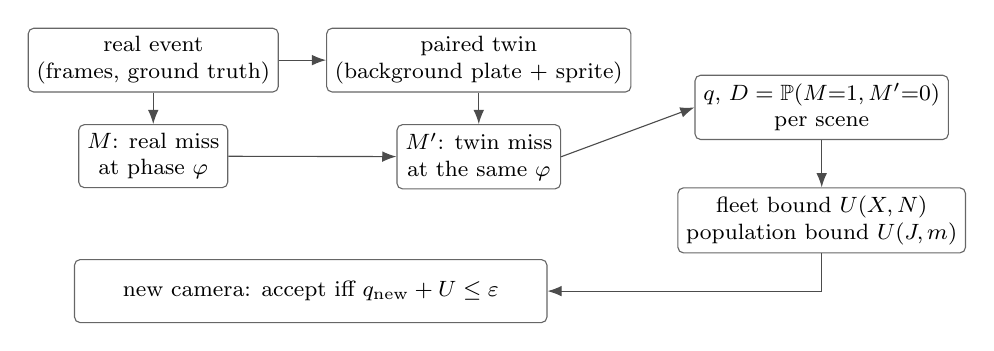
\begin{tikzpicture}[font=\footnotesize, node distance=4mm and 6mm,
  box/.style={draw=black!60, rounded corners=2pt, align=center, inner sep=3pt, minimum height=8mm},
  arr/.style={-{Latex[length=1.8mm]}, draw=black!70}]
\node[box] (real) {real event\\(frames, ground truth)};
\node[box, right=of real] (twin) {paired twin\\(background plate + sprite)};
\node[box, below=of real] (M) {$M$: real miss\\at phase $\varphi$};
\node[box, below=of twin] (Mp) {$M'$: twin miss\\at the same $\varphi$};
\node[box, right=8mm of twin, yshift=-6mm] (qd) {$q$, $D=\PP(M{=}1,M'{=}0)$\\per scene};
\node[box, below=of qd, yshift=-2mm] (cert) {fleet bound $\UCP(X,N)$\\population bound $\UCP(J,m)$};
\node[box, below=9mm of M, xshift=20mm, minimum width=60mm] (dec) {new camera: accept iff $q_{\mathrm{new}}+\UCP\le\varepsilon$};
\draw[arr] (real) -- (twin);
\draw[arr] (real) -- (M);
\draw[arr] (twin) -- (Mp);
\draw[arr] (M) -- (Mp);
\draw[arr] (Mp.east) -- (qd.west);
\draw[arr] (qd) -- (cert);
\draw[arr] (cert.south) |- (dec.east);
\end{tikzpicture}
\caption{The demonstration with a paired twin. Each real event is paired with a synthetic twin that replaces the object and
keeps the scene; both are evaluated by the same detector at the same sampling phase. Discordances calibrated across scenes
bound the miss probability of a new camera through $p\le q+D$.}
\label{fig:scheme}
\end{figure}

% RESS Sections 5-8, derived from body.tex (TNNLS version) by P4 R3 script; edit here from now on.
% =====================================================================================================
\section{Experimental protocol}\label{sec:protocol}

\paragraph{Data} The corpus is rebuilt from the raw detections and pixel ground truth of CDnet 2014~\cite{cdnet2014} and
LASIESTA~\cite{lasiesta2016} (frames in true temporal order), with the synthetic part of the BMC benchmark~\cite{bmc2012} as an
off-the-shelf simulator; the detector-defined corpus has \nCorpusT{} events from \nCorpusTvideos{} real videos. For the
twin we use ground-truth events: a frame is a \emph{hit} if a detector box covers at least half of the largest
ground-truth component or overlaps its bounding box with IoU $\ge0.3$, and an event counts if its largest object has at
least 256 pixels (primary definition; the original definition keeps every ground-truth event). Scenes are assigned
to tiers by the category labels of the two datasets. The \emph{static} (main) domain is every CDnet calibration scene
outside the categories \emph{PTZ}, \emph{cameraJitter}, \emph{nightVideos} and \emph{turbulence}, and every LASIESTA
calibration scene outside the categories SM (simulated camera motion) and MC (moving camera): \nMainScenes{} scenes
(\nMainCDnet{} CDnet, \nMainLASIESTA{} LASIESTA; \nDefAllA{} events of any duration, \nMainN{} of at least 32 frames).
The other tiers are night (\nNightScenes{} scenes), turbulence (\nTurbScenes{} scenes; only 2 were run and they hold
\nTurbN{} events, so the tier is reported but not certified) and camera jitter (\nJitterScenes{} scenes: CDnet
\emph{cameraJitter} and LASIESTA SM); the \nPTZScenes{} pan-tilt-zoom and \nMCScenes{} moving-camera scenes are
excluded, because the twin assumes a static background. This definition was fixed after the initial version of this
study, whose static domain was wider; no twin or detector was re-run, and the supplement compares the static domain
of the three versions (Table~S\SuppTabVersions).

\paragraph{Detector and twin} The detector is a fixed single-stage segmentation network (YOLO family~\cite{redmon2016};
yolo26s-seg~\cite{ultralytics}, confidence 0.25, input 640 px, CPU). Per scene, a background plate is the per-pixel median
of up to 60 frames without ground-truth foreground. For each real event and each of three sprite variants (fixed
seeds), the twin removes the real object (mask dilated by 3 px), fills it from the plate, and draws a synthetic object
on the ground-truth trajectory: a vehicle cut from Virtual KITTI~2~\cite{cabon2020vkitti2}, chosen by aspect ratio, or
a procedurally dressed human rendered with MPFB~\cite{mpfb2} with a four-frame walking cycle mirrored to the motion
direction. The sprite height equals the ground-truth box height, its width is clamped to $\pm10\%$ of the box width, its
brightness follows the frame luminance, and a soft shadow is added. Only the object is synthetic; scene, illumination
and background clutter are real. The detector runs on twin frames until the twin hits cover all residues modulo 48,
which is exact for every $K$ dividing 48. The median detector confidence on twin hits is \nConfTwin{} (real:
\nConfReal). Building the twins of the \nMainScenes{} static scenes took \nTwinCostTotal{} CPU-hours (median \nTwinCostScene{} per
scene) on a laptop CPU.

\paragraph{What the twin consumes} The paired twin uses, per camera, empty frames (for the plate) and the annotated
trajectories of the camera's real events (for sprite placement). Calibration therefore costs annotated events:
\nMainN{} at \OPs, i.e.\ \nCalibPerCam{} per static camera when amortized over the domain. For a \emph{new} camera, the
exchange rates below assume that the twin miss rate $q_{\mathrm{new}}$ can be measured without that camera's real
events, e.g.\ with synthetic trajectories drawn on its empty background. We did not build such trajectory-free twins;
we use the paired $q_s$ in their place. The discordance of a trajectory-free twin has not been calibrated, so the
reported savings are conditional on the paired-twin discordance carrying over, and are upper bounds.

\paragraph{Operating points} An operating point is $(\varepsilon,d_{\min},K)$ with events of at least $d_{\min}$
frames. The primary point \OPs{} $=(20\%, 32, 16)$ at $\delta=5\%$ was fixed by a rule chosen before the twin was built
(the largest $K$ for which direct certification needs at most 150 events at 80\% power and the 44 calibration scenes
available at that time give a population bound of at most $\varepsilon/2$), using the pooled real miss rate of all
CDnet events of every category (\nOldPhat{} over \nOldN{} such events, \nOldNreq{} events for direct certification). In the static domain the real miss rate at \OPs{} is only
\nPmainOP; we report this, keep \OPs, and add the sensitivity points OP-A $(20\%,32,8)$ and OP-C $(10\%,32,1)$ and the
full grid $d_{\min}\in\{1,4,8,12,16,24,32\}$, $K\in\{1,2,3,4,6,8,12,16,24,48\}$. The night and turbulence tuning criteria and their held-out
scenes were fixed before tuning. These choices are dated in internal project records but were not publicly registered.
Six choices were made after results were available and are disclosed: (i) the primary event definition (largest
object at least 256 pixels) was adopted after the initial twin run, with the original definition kept as a co-reported
sensitivity (Table~\ref{tab:eventdef}); (ii) the list of LASIESTA calibration scenes, before the split into tiers, was rebuilt (20 to 48 scenes) after correcting
the frame order of that dataset, before the twin was built; (iii) the two held-out turbulence scenes were not run;
(iv) the CDnet \emph{cameraJitter} scenes and (v) the LASIESTA SM and MC scenes were removed from the static domain
after static-domain results were available; and (vi) a second operating point with more real misses was examined after
inspecting the data (Section~\ref{sec:audit}). The operating point \OPs, the audit design and the night criterion were
fixed before the static-domain twin results; everything else in Section~\ref{sec:results} is exploratory.

\paragraph{Why a paired twin} A reweighting alternative~\cite{shimodaira2000} needs overlap between synthetic and real
events. A classifier separating BMC events from real events reaches a median AUC of \nIWtemporal{} with temporal
features, \nIWgeometry{} with geometry and \nIWappearance{} with detector confidence alone (all targets); the gap lies
mostly in geometry, so a reweighted synthetic benchmark cannot stand in for the real event distribution, and the twin
is matched on geometry by construction.

\paragraph{Audit} Leave-one-scene-out (LOSO): each scene is certified with the bound computed from the other scenes.
Monte Carlo (10{,}000 draws): calibration scenes are resampled from the static domain and a new camera is drawn from it;
a false certificate is a certified camera with $p_s>\varepsilon$ (the resampled calibration set may contain the test
camera, which makes this check optimistic; the LOSO audit does not have this defect); the ``truth'' of a camera is its own event pool,
exact over phases. Two must-fail scenarios are run (Section~\ref{sec:audit}). All randomness uses seed 42.

% =====================================================================================================
\section{Results}\label{sec:results}

\subsection{Certificates by tier}
In the static domain, \nMainDw{} of \nMainN{} events at \OPs{} are discordant; hence $\UCP(X,N)=\nMainUfleet$ and,
with $J=\nMainJ$ of \nMainM{} scenes, $\UCP(J,m)=\nMainUpop$ (Table~\ref{tab:tiers}, Fig.~\ref{fig:tiers}). Both are
below $\varepsilon/2=10\%$. In the camera-jitter tier, \nJitDw{} of \nJitN{} events are discordant, all in the CDnet
scene \emph{traffic}, which has real camera shake; the LASIESTA scenes with simulated camera motion have no discordant
event. At
night, \nNightDw{} of \nNightN{} events are discordant (\nNightDwPct; phase-averaged \nNightDexp) and \nNightJ{} of
\nNightScenes{} scenes; pooling all tiers raises the bounds to \nAllUfleet{} and \nAllUpop.

\begin{table}[t]
\centering
\caption{Certificates by tier at \OPs{} ($\delta=5\%$). Discordant events are counted at the worst sampling phase
(in parentheses: phase-averaged count, mean over the three sprite variants; per-scene tables use the majority rule, which
gives \nNightDexpMaj{} at night); $\hat p$, $\hat q$: real and twin miss rates averaged over the phases / at the worst
phase (any fixed deployment phase); $J$ = scenes with a discordant event.}
\label{tab:tiers}
\footnotesize
\setlength{\tabcolsep}{2.5pt}
\begin{tabular}{@{}lrrrrrrr@{}}
\toprule
tier & events & $\hat p$ avg/worst & $\hat q$ avg/worst & discordant & $\UCP(X,N)$ & $J/m$ & $\UCP(J,m)$ \\
\midrule
static (main) & \nMainN & \nPASpMain/\nWPSpMain & \nPASqMain/\nWPSqMain & \nMainDw{} (\nMainDexp) & \nMainUfleet & \nMainJ/\nMainM & \nMainUpop \\
camera jitter & \nJitN & \nPASpJit/\nWPSpJit & \nPASqJit/\nWPSqJit & \nJitDw & \nJitUfleet & \nJitJ/\nJitM & \nJitUpop \\
night & \nNightN & \nPASpNight/\nWPSpNight & \nPASqNight/\nWPSqNight & \nNightDw{} (\nNightDexp) & \nNightUfleet & \nNightJ/\nNightScenes & \nNightUpop \\
turbulence & \nTurbN & \nPASpTurb/\nWPSpTurb & \nPASqTurb/\nWPSqTurb & \nTurbDw & \nTurbUfleet & \nTurbJ/\nTurbM & \nTurbUpop \\
all tiers & \nAllN & \nPASpAll/\nWPSpAll & \nPASqAll/\nWPSqAll & \nAllDw & \nAllUfleet & \nAllJ/\nAllM & \nAllUpop \\
\bottomrule
\end{tabular}
\end{table}

\begin{figure}[t]
\centering
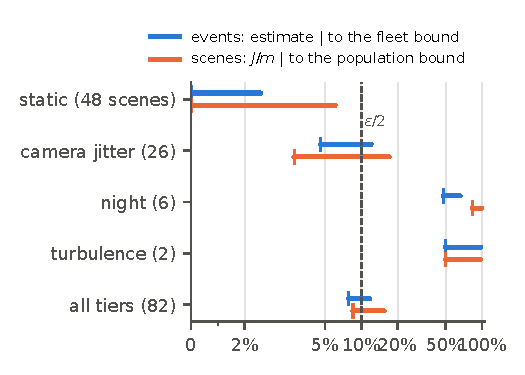
\includegraphics[width=0.8\textwidth]{figs/fig_tiers.pdf}
\caption{Certificates by tier at \OPs{} (event unit, worst phase). Blue: discordant events per event and the fleet bound; orange: discordant scenes per scene and the population bound. Dashed: $\varepsilon/2$.}
\label{fig:tiers}
\end{figure}

\subsection{Exchange rate}\label{sec:exchange}
Fig.~\ref{fig:exchange} and Table~\ref{tab:grid} show the real events a static camera saves when the twin replaces
direct certification, across \nGridPts{} operating points. A camera is certified with no real event when its twin miss
rate plus the transfer bound (both at $\delta/2$, the bound computed without the camera) stays below $\varepsilon$. At
\OPs{} the direct test needs only $n_0=\nNzeroTwenty$ events, because the static-domain miss rate is low; a twin run to
convergence saves those \nSavedOP{} events at \nSavedCamOP{} of \nMainScenes{} cameras, at a measured cost of \nCpuPerSavedOP{}
CPU-hours per saved event (conditional on the discordance carrying over, Section~\ref{sec:protocol}; no accepted camera
has $p_s>\varepsilon$ at \OPs, but acceptances were not audited at every grid cell). \textbf{The twin as built saves no
real events; the saving requires about \nTwinRunsOP{} twin
runs per camera.} With three runs per event, as built, the twin's own miss rate cannot be bounded tightly enough, and at
most \nGridFinMax{} cameras save anything at any grid point. The saving grows with the real miss rate, because direct
certification becomes expensive: it reaches hundreds of events per camera at some grid cells with $\hat p$ above
$10\%$, while at $K=48$ and closer to $\varepsilon$ the twin route saves nothing (Table~\ref{tab:grid}). The target $\varepsilon=20\%$ is a demonstrator, not a safety target. At
$\varepsilon=5\%$ the domain rule requires a population bound of at most $\varepsilon/2=2.5\%$, which needs at least
\nPopScenesQuarter{} calibration scenes even with no discordant scene; with \nMainScenes{} scenes the twin route is not
available at $\varepsilon=5\%$, whatever the twin budget. For the calibrated cameras
themselves, direct Clopper--Pearson on their pooled real misses gives \nDirectPooledU, close to the fleet discordance
bound \nMainUfleet: the fleet certificate adds little where real data exist, and its role is as the building block of
the transfer.

\begin{figure}[t]
\centering
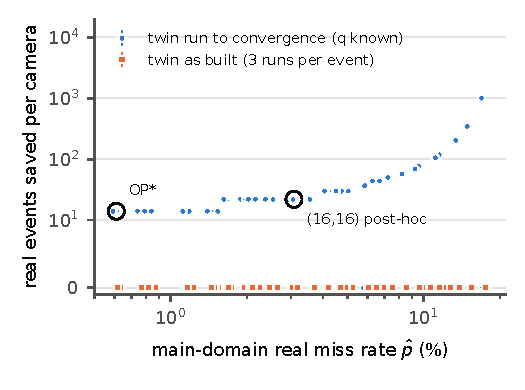
\includegraphics[width=0.8\textwidth]{figs/fig_exchange_rate.pdf}
\caption{Exchange rate: real events saved per static camera (median and interquartile range over \nMainScenes{} cameras) against
the static-domain real miss rate, one point per $(d_{\min},K)$ at $\varepsilon=20\%$. Blue: twin run to convergence;
orange: twin as built (three runs per event). Vertical axis: symmetric log (linear below 10). Circled: \OPs.}
\label{fig:exchange}
\end{figure}

\begin{table}[t]
\centering
\caption{Exchange rate at three operating points (\nMainScenes{} static cameras). $n_{\mathrm{dir}}$: real events of the smallest direct
plan (failures allowed, Clopper--Pearson acceptance) with 80\% power at the pooled static-domain $\hat p$; the
zero-failure plan alone needs $n_0$ events; saved: median real events saved per camera by a twin run to
convergence; runs: twin runs needed per camera; CPU-h: CPU-hours per saved real event.}
\label{tab:exchange}
\setlength{\tabcolsep}{4pt}
\begin{tabular}{@{}lrrrrrr@{}}
\toprule
point & $\hat p$ & $n_{\mathrm{dir}}$ & saved & cams & runs & CPU-h \\
\midrule
\OPs{} $(20\%,32,16)$ & \nTpOPS & \nTndOPS & \nTsvOPS & \nTcamOPS & \nTrunsOPS & \nTcpuOPS \\
OP-A $(20\%,32,8)$ & \nTpOPA & \nTndOPA & \nTsvOPA & \nTcamOPA & \nTrunsOPA & \nTcpuOPA \\
OP-C $(10\%,32,1)$ & \nTpOPC & \nTndOPC & \nTsvOPC & \nTcamOPC & \nTrunsOPC & \nTcpuOPC \\
\midrule
\multicolumn{7}{@{}l}{worst-phase convention (valid for any fixed phase):}\\
\OPs{} & \nWXSp & \nWXSnd & \nWXSsaved & \nWXSacc & \nWXSruns & -- \\
\midrule
\multicolumn{7}{@{}l}{twin as built: cameras saving $=$ \nTcamfinOPS, \nTcamfinOPA, \nTcamfinOPC{} (median saving 0)}\\
\bottomrule
\end{tabular}
\end{table}

\begin{table}[t]
\centering
\caption{Operating-point grid at $\varepsilon=20\%$ (condensed; full grid in the supplement). Each cell: static-domain real miss rate $\hat p$ / real events for direct certification / median real events saved per camera by a twin run to convergence. The twin as built saves none at every cell. OP$^\ast$ is $(32,16)$.}
\label{tab:grid}
\scriptsize
\setlength{\tabcolsep}{3pt}
\begin{tabular}{@{}rccccc@{}}
\toprule
$d_{\min}\backslash K$ & 1 & 8 & 16 & 24 & 48 \\
\midrule
32 & 0.6\%/14/14 & 0.6\%/14/14 & 0.6\%/14/14 & 0.8\%/14/14 & 4.1\%/30/0 \\
24 & 0.6\%/14/14 & 0.7\%/14/14 & 1.2\%/14/14 & 1.6\%/22/22 & 5.8\%/37/0 \\
16 & 1.1\%/14/14 & 1.9\%/22/22 & 3.1\%/22/22 & 4.4\%/30/30 & 9.7\%/76/0 \\
12 & 1.7\%/22/22 & 2.4\%/22/22 & 3.6\%/22/22 & 4.9\%/30/30 & 10.2\%/88/0 \\
8 & 1.6\%/22/22 & 2.9\%/22/22 & 5.0\%/30/30 & 6.7\%/44/44 & 12.2\%/141/0 \\
4 & 2.0\%/22/22 & 6.3\%/44/44 & 9.5\%/76/76 & 11.5\%/118/118 & 17.2\%/1164/0 \\
1 & 2.4\%/22/22 & 11.1\%/106/106 & 14.9\%/348/348 & 16.9\%/1006/1006 & 22.4\%/--/0 \\
\bottomrule
\end{tabular}
\end{table}


\subsection{Audit and must-fail scenarios}\label{sec:audit}
\emph{Is the certificate right because it is empty?} Table~\ref{tab:confusion} cross-tabulates real and twin outcomes.
In the static domain at \OPs{} almost every event is caught by both: \nRealMissEvOP{} events have a real miss at some
phase, in \nRealMissScOP{} scenes, and the twin also misses \nRecallOP{} of the expected real misses, i.e.\ one event.
The zero-discordance result is therefore mostly a statement about a detector that rarely misses in this domain, not a
test of the twin. At night the twin sees almost none of the real misses.

\begin{table}[t]
\centering
\caption{Real versus twin outcomes (expected event counts under a uniform sampling phase; twin = majority of three variants). Recall: share of expected real misses that the twin also misses. \textsuperscript{ph}\,post hoc.}
\label{tab:confusion}
\scriptsize
\setlength{\tabcolsep}{3pt}
\begin{tabular}{@{}lrrr@{}}
\toprule
 & static, OP$^\ast$ & static, $(16,16)$\textsuperscript{ph} & night, OP$^\ast$ \\
\midrule
real miss, twin miss & 1.00 & 4.81 & 0.75 \\
real miss, twin catch ($D$) & 0.31 & 1.94 & 8.31 \\
real catch, twin miss & 0.56 & 3.62 & 0.44 \\
real catch, twin catch & 178.12 & 189.62 & 15.50 \\
\midrule
events & 180 & 200 & 25 \\
events missed at some phase & 4 & 20 & 13 \\
twin recall of real misses & 76\% & 71\% & 8\% \\
\bottomrule
\end{tabular}
\end{table}


\emph{LOSO and Monte Carlo.} At \OPs, the number of static scenes whose discordance exceeds the bound computed
without them is \nLosoOP{} of \nMainScenes{} (Fig.~\ref{fig:loso}); the Monte-Carlo
false-certification rate is \nMcFC. Because real misses are rare at \OPs, this audit cannot reveal much: only
\nScenesPgtEpsOP{} static scene has $p_s>\varepsilon$ there (the one holding the single missed event), and it is refused, so
the 0\% rate rests on that one scene.
A scene above its leave-one-out bound would still be compatible with a population-average guarantee. The informative
tests are must-fail~2 and the camera-jitter check below, which can fail and do.

\emph{Must-fail 1: temporal.} At $K=48$, \nMustFailScenes{} static scenes have $p_s>\varepsilon$ and the procedure refuses
them in \nMustFailRefuse{} of runs; but most of these misses are temporal (events shorter than $K$, which the twin
reproduces by construction); the number of scenes that exceed $\varepsilon$ through detector misses is \nMustFailApp
(Table~\ref{tab:mustfail}, top).

\emph{Must-fail 2: detector.} We add $k$ of the 6 night scenes to the calibration as if they were static-domain scenes;
at \OPs{} every real miss of these scenes is a detector miss. The transfer bound rises with $k$
(Fig.~\ref{fig:leak}, Table~\ref{tab:mustfail}, bottom): from \nLeakUpopZero{} to \nLeakUpopSix{} at \OPs{}, crossing
$\varepsilon/2$ for some subsets at $k=\nLeakWithdrawKfirst$ and for all at $k=\nLeakWithdrawK$, so the domain-level
certificate is withdrawn; no static camera is ever falsely certified (\nMainFCleak). \emph{Out-of-domain pass-through:}
the per-camera rule does not protect the night cameras themselves. The night twin misses almost nothing (its appearance
model only dims the sprite), so each night camera, judged with a bound computed from the static scenes, is certified;
\nNightFC{} of \nNightScenes{} night cameras have $p_s>\varepsilon$ and are falsely certified at \OPs{}
(Table~\ref{tab:mustfail}, middle). Each night miss rate rests on 2 to 10 events and is uncertain; the
finding is that the acceptance rule admitted these cameras although their observed miss rates exceed $\varepsilon$ and
their twins miss almost nothing, not a precise estimate of their miss rates.

\emph{Camera jitter.} The same pass-through occurs for a shaking camera, but it rests on a single scene. Judged by the
twin route calibrated on the static scenes (worst-phase convention, Section~\ref{sec:checks}), \nOODSJitacc{} of the
\nOODSJitcams{} camera-jitter cameras are accepted and \nOODSJitfa{} of them is falsely accepted: \emph{traffic}, a
CDnet scene with real camera shake, whose worst-phase real miss rate is \nOODSJitFApw{} (per-camera table in the
supplement). Its twin catches every event at every phase, because the synthetic object is drawn on a stabilised plate
while the real frames shake; under the phase-averaged reading this camera stays below $\varepsilon$
(Table~\ref{tab:mustfail}, camera-jitter rows), so this failure appears only for a fixed deployment phase. The
LASIESTA scenes with simulated camera motion produce no discordance and no false acceptance, so they add little
evidence either way about real shake. Under the same worst-phase rule \nOODSNightfa{} of
\nOODSNightcams{} night cameras are falsely accepted at \OPs.

\begin{table}[t]
\centering
\caption{Must-fail scenarios. Top: temporal ($d_{\min}=1$, $K=48$), static scenes with $p_s>\varepsilon$, real misses split into detector and temporal misses; all refused in every Monte-Carlo run. Middle: night scenes at OP$^\ast$ (every miss is a detector miss), and whether each is falsely certified when judged alone (phase-averaged); then the same for the camera-jitter scenes. Bottom: population bound when $k$ night scenes leak into the calibration set (median over subsets; withdrawn = share of subsets with a bound above $\varepsilon/2$).}
\label{tab:mustfail}
\scriptsize
\setlength{\tabcolsep}{3pt}
\begin{tabular}{@{}lrrrrrr@{}}
\toprule
\multicolumn{7}{@{}l}{\emph{1: temporal}} \\
scene & $n$ & $p_s$ & detector & temporal & $q_s$ & refused \\
\midrule
port\_0\_17fps & 5 & 99.6\% & 43.3\% & 56.2\% & 100.0\% & 100\% \\
tramCrossroad\_1fps & 11 & 77.7\% & 6.1\% & 71.6\% & 74.2\% & 100\% \\
tunnelExit\_0\_35fps & 34 & 83.6\% & 5.2\% & 78.4\% & 87.9\% & 100\% \\
\midrule
\multicolumn{7}{@{}l}{\emph{2: detector (night)}} \\
scene & $n$ & $p_s$ & $q_s$ & $D_s$ & disc. & false cert. \\
\midrule
bridgeEntry & 2 & 15.6\% & 0.0\% & 15.6\% & 1 & no \\
busyBoulvard & 4 & 96.9\% & 0.0\% & 96.9\% & 4 & yes \\
fluidHighway & 4 & 26.6\% & 0.0\% & 26.6\% & 2 & yes \\
streetCornerAtNight & 10 & 28.1\% & 11.9\% & 20.6\% & 4 & yes \\
tramStation & 2 & 0.0\% & 0.0\% & 0.0\% & 0 & no \\
winterStreet & 3 & 33.3\% & 0.0\% & 33.3\% & 1 & yes \\
\midrule
\multicolumn{7}{@{}l}{\emph{3: detector (camera jitter)}} \\
\midrule
boulevard & 8 & 0.0\% & 0.0\% & 0.0\% & 0 & no \\
traffic & 8 & 3.9\% & 0.0\% & 3.9\% & 3 & no \\
\midrule
$k$ leaked & 0 & 1 & 2 & 3 & 4 & 6 \\
\midrule
$U_{\mathrm{pop}}$ & 3.9\% & 6.0\% & 7.9\% & 8.6\% & 9.4\% & 12.4\% \\
withdrawn & 0\% & 0\% & 0\% & 0\% & 33\% & 100\% \\
\bottomrule
\end{tabular}
\end{table}


\begin{figure}[t]
\centering
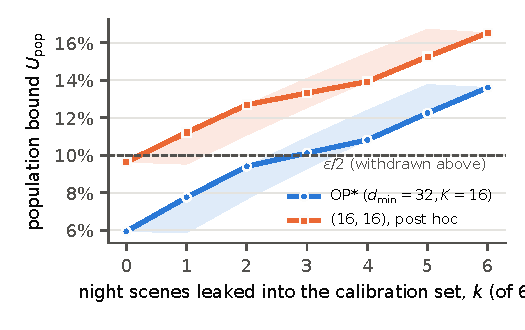
\includegraphics[width=0.8\textwidth]{figs/fig_leak.pdf}
\caption{Must-fail 2: the population bound when $k$ night scenes leak into the static calibration set (median over the
$\binom{6}{k}$ subsets, band: min--max). The domain certificate is withdrawn above $\varepsilon/2$. Individual night
cameras are still certified when judged alone (out-of-domain pass-through, text).}
\label{fig:leak}
\end{figure}

\begin{figure}[t]
\centering
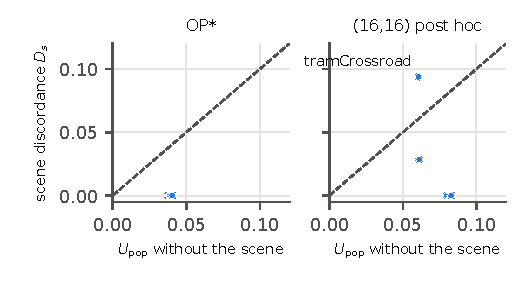
\includegraphics[width=0.8\textwidth]{figs/fig_loso.pdf}
\caption{Leave-one-scene-out: per-scene discordance against the population bound computed without the scene. Points above
the diagonal exceed the bound; the proposition bounds the population mean, not each scene.}
\label{fig:loso}
\end{figure}

\emph{A post-hoc operating point.} To see the certificate under more real misses, the point $(d_{\min},K)=(16,16)$ was
examined after inspecting the data; it fails the criterion we fixed before recomputing it on the static domain (both
bounds at most $\varepsilon/2$ and no false acceptance), because its population bound is \nWPCUpMain, and it is not
reported further.

\subsection{Fixed-phase and site-level checks}\label{sec:checks}
\emph{Worst phase.} A deployed camera keeps one sampling phase. Counting an event as missed if it is missed at any
phase, for the real event, the twin (majority of variants) and the discordance alike, keeps the bound valid for every
fixed phase, because an event missed at some phase is either missed by the twin or discordant at that phase. At \OPs{}
the static-domain real and twin miss rates become \nWPSpMain{} and \nWPSqMain{} (phase-averaged \nPASpMain{} and
\nPASqMain), while the discordance counts and both bounds are unchanged (Table~\ref{tab:tiers}). The direct plan then
needs \nWXSnd{} events, and a twin run to convergence accepts \nWXSacc{} of \nMainScenes{} cameras, saving \nWXSsaved{}
events each (Table~\ref{tab:exchange}); the number of accepted static cameras with a worst-phase real miss rate above
$\varepsilon$ is \nWXSfa.

\emph{Sites.} Scenes filmed at the same site share background, viewpoint and illumination, so the scene may be too fine
a unit of independence. Grouping the static scenes into \nSiteSm{} sites (CDnet challenge categories and LASIESTA
sequence groups, a coarse proxy for sites), the number of sites with a discordant event at \OPs{} is \nSiteSJ, yet
with so few units the population bound is $\UCP(J_{\mathrm{site}},m_{\mathrm{site}})=\nSiteSU$, above $\varepsilon/2$:
under the domain rule the transfer claim is withdrawn at site level. The leave-one-site-out audit finds \nSiteSloso{}
sites above their bound at \OPs. The transfer certificate therefore stands at scene level and is withdrawn at site level; it holds only if
scenes, not sites, are the independent units.

\subsection{Failure modes}
At night the twin sees few real misses: it predicts \nRecallNight{} of the expected missed events, and the tier bound is
\nNightUpop. Fig.~\ref{fig:sprites} shows why: the appearance model scales sprite brightness with the scene, but has no
headlights, glare or sensor noise. An attempt to fix this was specified in advance: night-specific appearance profiles were
tuned on four night scenes and judged on two held-out scenes, with success defined as a median held-out per-scene
discordance of at most 5\%. The best profile barely moved the tuning discordance (\nNightBaseD{} to \nNightProfD,
phase-averaged) and the held-out median was \nNightHeldD{} on \nNightHeldN{} events, so the criterion failed, tuning was
stopped, and night is declared outside the domain. Camera jitter is the second named failure mode, observed in one
scene with real shake: the twin is drawn on a stabilised background plate, so it cannot reproduce the misses caused by
camera shake (over the tier, twin worst-phase miss rate \nWPSqJit{} against a real \nWPSpJit{} at \OPs;
Table~\ref{tab:tiers}). One scene does not show how often real shake produces this failure. The turbulence tier holds
\nTurbN{} events at \OPs{} and is not certified.

\begin{figure}[t]
\centering
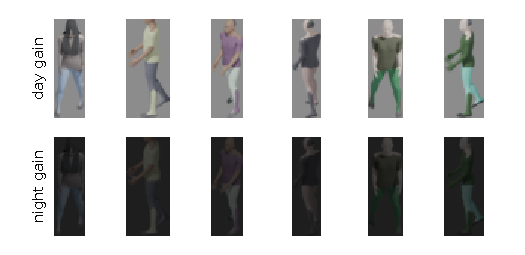
\includegraphics[width=0.8\textwidth]{figs/fig_sprites.pdf}
\caption{Synthetic person sprites (CC0) on a neutral background under the brightness gain used for day and for night
scenes. Dimming alone does not reproduce night imaging, which explains the low twin miss rate at night.}
\label{fig:sprites}
\end{figure}

\subsection{Sensitivity}
\emph{Event definition.} Keeping every ground-truth event (\nDefAllO{} instead of \nDefAllA{} static events of any
duration) leaves \OPs{} almost unchanged: \nOrigN{} events, \nOrigOPDw{} discordant, $\UCP(X,N)=\nOrigOPUfleet$, $J=\nOrigJ$
(Table~\ref{tab:eventdef}).
\emph{Operating point.} At OP-A and OP-C the static-domain miss rate is \nPmainOPA{} and \nPmainOPC{}, and no
static-domain event is discordant.
\emph{Twin details.} The majority rule over sprite variants (1, 2 or 3 of 3) does not change any static-domain count.
Table~\ref{tab:fidelity} compares twin and real hit rates on the same frames: the twin is pessimistic at every
aspect error except one vehicle bin, and both hit rates fall when the ground-truth box has an unusual aspect (occlusion,
objects entering the frame). Clamping the sprite width, which affects \nClampShare{} of twin frames (more than the frames with an aspect error
above 10\% in Table~\ref{tab:fidelity}, because 1-pixel rounding also triggers the clamp), lowers the twin hit
rate by only \nClampExtraDrop{} points more than the real hit rate on the same frames (\nClampPairs{} event--variant
pairs): it inflates $q$, not $D$. The median detector confidence on hits is lower for the twin than for real objects,
especially for persons. Full tables are in the supplement.

\begin{table}[t]
\centering
\caption{Twin fidelity on the same frames (static domain): hit rates by object kind and sprite aspect error before the width clamp, and median detector confidence on hits. Negative differences make the twin pessimistic.}
\label{tab:fidelity}
\scriptsize
\setlength{\tabcolsep}{3pt}
\begin{tabular}{@{}llrrrr@{}}
\toprule
kind & $|$aspect error$|$ & frames & twin hit & real hit & diff.\ (pts) \\
\midrule
person & $\le$10\% & 8,870 & 91.7\% & 94.8\% & -3.2 \\
person & 10-20\% & 5,899 & 90.1\% & 94.2\% & -4.2 \\
person & 20-40\% & 4,404 & 74.0\% & 86.2\% & -12.2 \\
person & $>$40\% & 5,449 & 34.4\% & 44.5\% & -10.0 \\
vehicle & $\le$10\% & 4,105 & 86.9\% & 89.0\% & -2.1 \\
vehicle & 10-20\% & 2,569 & 88.0\% & 90.2\% & -2.2 \\
vehicle & 20-40\% & 3,087 & 87.6\% & 85.1\% & +2.5 \\
vehicle & $>$40\% & 3,881 & 64.9\% & 74.2\% & -9.3 \\
\midrule
person & confidence & & 0.86 & 0.92 & \\
vehicle & confidence & & 0.72 & 0.78 & \\
\bottomrule
\end{tabular}
\end{table}


\begin{table}[t]
\centering
\caption{Event-definition sensitivity (static domain). Primary: largest object $\ge 256$ px; original: every ground-truth event. Discordant events at the worst phase; LOSO: scenes above the bound computed without them.}
\label{tab:eventdef}
\scriptsize
\setlength{\tabcolsep}{3pt}
\begin{tabular}{@{}llrrrrrr@{}}
\toprule
definition & point & $N$ & $\hat p$ & disc. & $\UCP(X,N)$ & $J$ / $\UCP(J,m)$ & LOSO \\
\midrule
primary & OP$^\ast$ & 114 & 0.88\% & 0 & 2.59\% & 0 / 6.1\% & 0 \\
 & OP-A & 114 & 0.88\% & 0 & 2.59\% & 0 / 6.1\% & 0 \\
 & OP-C & 114 & 0.88\% & 0 & 2.59\% & 0 / 6.1\% & 0 \\
\midrule
original & OP$^\ast$ & 116 & 0.86\% & 0 & 2.55\% & 0 / 6.1\% & 0 \\
 & OP-A & 116 & 0.86\% & 0 & 2.55\% & 0 / 6.1\% & 0 \\
 & OP-C & 116 & 0.86\% & 0 & 2.55\% & 0 / 6.1\% & 0 \\
\bottomrule
\end{tabular}
\end{table}


% =====================================================================================================
\section{Discussion and limitations}\label{sec:discussion}

\emph{A narrow window.} Simulation pays in events only when direct certification is expensive, that is, when the real
miss rate is not far below $\varepsilon$; there the twin must also be accurate, and discordances make the transfer bound
grow. When the miss rate is low, $n_0$ is small and there is little to save. The grid (Table~\ref{tab:grid}) shows both
ends: \nNzeroTwenty{} events at \OPs, hundreds at some operating points with $\hat p$ above $10\%$, and nothing
where $\hat p$ comes close to $\varepsilon$.

\emph{Time.} The waiting time saved at camera $s$ is $n_{\mathrm{saved}}/\lambda_s$, where $\lambda_s$ is the event rate
in deployment; we do not estimate it, because the benchmarks publish no frame rates and their clips are dense in events.
If one CPU-hour is valued like one hour of waiting, the twin breaks even when $\lambda_s<1/c\approx\nBreakEven$ events per
hour at \OPs{}, with $c$ the CPU-hours per saved event; this equivalence is an assumption, not a measurement.

\emph{Domain.} The transfer bound is a population-average guarantee: it withdraws the domain certificate when
out-of-domain scenes enter the calibration, but it does not detect an out-of-domain camera. The domain must therefore be
declared and checked by other means (for example, illumination statistics), and a per-camera guarantee requires the
data of Result~4(c). Three items are left for future work: a twin that needs no annotated real trajectory of the new camera, with its own
calibrated discordance; a pre-specified in-domain stress test with cameras whose real miss rate exceeds $\varepsilon$;
and a domain check (for example a per-camera discordance sentinel on a few real events) to stop out-of-domain
pass-through.

\emph{Data and twin.} No static scene has 59 or more qualifying events, so per-camera ground truth is the scene's own
finite event pool; the twin builds its plate from real empty frames and therefore needs a static background; the sprite
library lacks elevated viewpoints for vehicles; and we did not use a full 3-D simulator. The operating point was fixed
from the pooled miss rate of all CDnet events, which turned out to be much higher than the static-domain rate; we kept it
rather than re-select after seeing the twin results. Scenes are not independent draws: several LASIESTA sequences share a room or set-up, and the site-level bound of
Section~\ref{sec:checks} exceeds $\varepsilon/2$. The
cost comparison counts real events and CPU-hours only; annotating the calibration events and building plates are
additional costs. Finally, an event miss is a component-level failure; linking it to a system hazard requires a
hazard analysis of the application.

\emph{Independence and phase.} The results assume independent events given the scene and independent scenes. Events
of one camera share a background, a detector and, in deployment, a single sampling phase; benchmark scenes are not a
random sample of deployments. Correlation of events within a scene does not invalidate the population bound of
Result~4(a) or the leave-one-scene-out audit, because both count scenes, not events: a scene contributes one
indicator whatever the dependence among its events. It does affect the fleet bound of Result~4(b), which counts
events and becomes optimistic under positive within-scene dependence; the population bound needs only independence
across scenes. The main results certify the phase-averaged miss rate; the worst-phase convention of Section~\ref{sec:checks} covers any
fixed phase at a higher real-event cost.

\emph{Threats to validity.} The audit tables and figures use level $\delta$, while acceptance uses $\delta/2$ for the
transfer term; at $\delta/2$ the bounds are larger (Result~4(a)). Software: Python 3.11.9, NumPy 1.26.4, SciPy 1.16.3,
pandas 2.3.3, Ultralytics 8.4.7, OpenCV 4.10.0; CPU: Intel Core i7-1185G7. The detector, the event definition and the
hit rule are fixed; a different detector changes
$p$, $q$ and $D$ but not the theorems. The number of scenes, not the number of events, limits the transfer certificate:
the static domain reaches $\UCP(J,m)=\nMainUpop$ with no discordant scene among \nMainM, and more scenes are needed for
tighter bounds. The audit at \OPs{} is weak because real misses are rare there. The label-based static domain was fixed after the initial version of this
study (Section~\ref{sec:protocol}); its clean audit is therefore partly a result of that post-hoc choice.

\emph{Practical guidance.} The results suggest a simple decision rule for practitioners who consider replacing a
field demonstration with a twin. (i) Compute $n_0$ at the target $(\varepsilon,\delta)$ and estimate the real miss rate;
if it is far below $\varepsilon$, the direct test is already short and a twin can save at most $n_0$ events. (ii) If a
twin is built, declare its domain before calibration and calibrate discordance on as many scenes of that domain as
possible; the number of scenes sets the resolution (Result~4(a)). (iii) Run each new camera's twin long
enough to bound its own miss rate; three runs per event, as here, are not enough. (iv) Do not use the transfer
certificate to admit a camera whose conditions differ from the calibration domain (night, a shaking mount): the
certificate is withdrawn when such scenes enter the calibration, but a single such camera passes through.

\section{Conclusion}\label{sec:conclusion}
Without an assumption linking simulation to reality, synthetic evidence buys no real events in zero-failure
certification, and relaxing the error level buys an exactly computable number. A paired twin turns the question into
one of discordance. The population bound is the transfer guarantee: it counts scenes, tolerates dependence within a
scene, and its price is the number of scenes; the fleet bound covers only the calibrated cameras and assumes independent
events. On the \nMainScenes{} static scenes of this study the transfer certificate stands at scene level
($\UCP(J,m)=\nMainUpop$) but is withdrawn at site level, where \nSiteSm{} sites give \nSiteSU, above $\varepsilon/2$.
Measured on public benchmarks, the exchange rate is modest and domain-bound; at $\varepsilon=5\%$ the transfer needs at
least \nPopScenesQuarter{} calibration scenes. The certificate has two named failure modes, night and camera jitter
(the latter seen in one scene with real shake), in which out-of-domain cameras pass through unless the domain is
declared.


\section*{CRediT authorship contribution statement}
\textbf{Lam Quoc Dat:} Conceptualization, Methodology, Software, Validation, Formal analysis, Investigation, Data
curation, Writing -- original draft, Writing -- review \& editing, Visualization.

\section*{Declaration of competing interest}
The author declares no competing interests. This research received no specific grant from any funding agency in the
public, commercial, or not-for-profit sectors.

\section*{Declaration of generative AI and AI-assisted technologies in the manuscript preparation process}
During the preparation of this work the author used an AI assistant (Claude, Anthropic) to write analysis and plotting
scripts, to check the numbers of the manuscript against the result files, and to draft and edit text. After using this
tool, the author reviewed and edited the content as needed and takes full responsibility for the content of the
publication.

\section*{Data availability}
Code, event manifests, result tables and the CC0 person-sprite set are publicly available at
\url{https://github.com/lamquocdat01/no-free-credit-ress-artifact} (tag \nRepoTag, commit \repohash). Raw video frames
(CDnet 2014, LASIESTA, BMC) and Virtual KITTI~2 sprites are not redistributed under their licences; the repository
provides download instructions and SHA-256 checksums to regenerate every derived file.

\appendix
\section{Formal statements and proofs}\label{app:proofs}
\renewcommand{\thetheorem}{A.\arabic{theorem}}
This appendix states the results of Section~\ref{sec:results-theory} formally and proves them. Theorem~\ref{thm:c1} is
Result~1, Theorem~\ref{thm:c2} is Result~2, Lemma~\ref{lem:c3} and Proposition~\ref{prop:c5a} are Result~3, and
Proposition~\ref{prop:pop}, Theorem~\ref{thm:fleet} and Proposition~\ref{prop:c4b} are Result~4(a), (b) and (c).
{\let\section\subsection
\renewcommand{\paragraph}[1]{\par\medskip\noindent\textbf{#1}\ }% run-in heading; titles carry their own period
% body of the proofs; \input by proofs_v1.tex and manuscript/supplement.tex
\section{Setting and notation}\label{sec:setting}

\paragraph{Events and misses.} A camera (scene) $s$ produces events $i=1,2,\dots$ (a maximal run of frames containing
the target object). The system samples frames periodically with period $K$ and an unknown phase
$\varphi\in\{0,\dots,K-1\}$; a detector is run on the sampled frames. An event is \emph{missed} ($M=1$) when no
sampled frame of the event is a hit (the detector finds the object). With $H\subseteq\mathbb{Z}$ the hit frames of
the event and $\varphi$ uniform, $\PP(M=1\mid H)=1-|H \bmod K|/K$, where $H\bmod K$ is the set of residues of $H$.
The miss rate of camera $s$ is $p_s=\PP(M=1)$ over its events and phases. Target: certify $p_s\le\varepsilon$ with
confidence $1-\delta$.

\paragraph{Clopper--Pearson bound.} For $x\in\{0,\dots,n\}$, $F_{n,p}(x)=\PP(\Bin(n,p)\le x)$ and
$\UCP(x,n)=\UCP_\delta(x,n)$ is the one-sided $(1-\delta)$ upper Clopper--Pearson bound
\cite{clopper1934}: the solution $u$ of $F_{n,u}(x)=\delta$ for $x<n$, and $1$ for $x=n$. Since $F_{n,p}(x)$ is
strictly decreasing in $p$, $\UCP(x,n)<p \iff F_{n,p}(x)<\delta$, and $\UCP$ is non-decreasing in $x$. Validity:
$\PP(\UCP(\Bin(n,p),n)<p)\le\delta$ for every $p$.

\paragraph{Success run.} $n_0(\varepsilon,\delta)=\lceil \ln\delta/\ln(1-\varepsilon)\rceil$ is the smallest $n$ with
$(1-\varepsilon)^n\le\delta$ (e.g.\ $n_0(5\%,5\%)=59$, $n_0(20\%,5\%)=14$).

\paragraph{Simulator and twin.} Simulator data $Y$ have a law $Q$ on an arbitrary space. A \emph{twin} is a paired
simulator: every real event $i$ has a synthetic counterpart with miss indicator $M'_i$ under the same sampling phase.
$q=\PP(M'=1)$, and the \emph{discordance} is $D=\PP(M=1,M'=0)$ (real miss, twin catch).

\section{C1: no free credit}

A certification procedure is a (possibly randomised) test $\phi(X,Y)\in\{0,1\}$ with real data
$X=(M_1,\dots,M_n)\sim\Bern(p)^{\otimes n}$ independent of simulator data $Y\sim Q$. It is \emph{valid at level
$\delta$ on a class $\mathcal{P}$} of pairs $(p,Q)$ if $\sup_{(p,Q)\in\mathcal{P},\,p>\varepsilon}\PP_{p,Q}(\phi=1)\le\delta$.

\begin{theorem}[C1]\label{thm:c1}
Assume $\mathcal{P}$ places no restriction linking $Q$ and $p$: for every $Q$ there are $(0,Q)\in\mathcal{P}$ and
$(p,Q)\in\mathcal{P}$ for all $p\in(\varepsilon,\varepsilon+\eta)$ for some $\eta>0$. If $\phi$ is valid at level
$\delta$ on $\mathcal{P}$, then for every $Q$ and every simulator sample size,
\[(1-\varepsilon)^n\,\PP_{0,Q}(\phi=1)\le\delta .\]
In particular, certifying a perfect system ($p=0$) with probability one requires $n\ge n_0(\varepsilon,\delta)$ real
events, whatever the amount of simulator data; power $1-\beta$ at $p=0$ requires
$n\ge \ln(\delta/(1-\beta))/\ln(1-\varepsilon)$.
\end{theorem}

\begin{proof}
Fix $Q$ and write $g(y)=\EE[\phi(0^n,y)]$ (expectation over the internal randomisation). Under $p=0$, $X=0^n$ almost
surely, so $\PP_{0,Q}(\phi=1)=\EE_Q[g(Y)]$. Under $p>\varepsilon$, the event $\{X=0^n\}$ has probability $(1-p)^n$ and
is independent of $Y$, hence $\PP_{p,Q}(\phi=1)\ge(1-p)^n\,\EE_Q[g(Y)]=(1-p)^n\PP_{0,Q}(\phi=1)$. Validity gives
$(1-p)^n\PP_{0,Q}(\phi=1)\le\delta$ for all $p\in(\varepsilon,\varepsilon+\eta)$; letting $p\downarrow\varepsilon$
proves the inequality. With $\PP_{0,Q}(\phi=1)=1$ it reads $(1-\varepsilon)^n\le\delta$, i.e.\ $n\ge n_0$; with
$\PP_{0,Q}(\phi=1)\ge 1-\beta$ it gives the power bound.
\end{proof}

\begin{remark}
The argument only uses that the simulator data have the same law under the two hypotheses and that the
all-success real sample has positive probability under both. It is the success-run analogue of the observation that
external data cannot increase power under strict type-I error control over all external-data laws
\cite{koppschneider2020}.
\emph{Check.} The zero-failure test with $n=59$ at $p=\varepsilon=5\%$: $(0.95)^{59}=\numConeClosed$ (MC
$\numConeMC$, $10^5$ runs).
\end{remark}

\section{C2: the price of borrowing}

Suppose one accepts a two-tier guarantee: level $\delta$ when the simulator is ``right'' and only level
$\delta'>\delta$ in general.

\begin{theorem}[C2, exact credit]\label{thm:c2}
(i) \emph{Converse.} Under the assumption of Theorem~\ref{thm:c1}, any procedure valid at level $\delta'$ on
$\mathcal{P}$ that certifies a perfect system with probability one uses $n\ge n_0(\varepsilon,\delta')$ real events.
Hence the credit, the number of real events saved with respect to $n_0(\varepsilon,\delta)$, is at most
\[c=n_0(\varepsilon,\delta)-n_0(\varepsilon,\delta').\]
(ii) \emph{Attainment.} Let $T(Y)\in\{0,1\}$ be any simulator test (``the simulator passes'') and let $B$ be the
procedure: if $T=1$ run the zero-failure test with $n_1=n_0(\varepsilon,\delta')$ real events, otherwise with
$n_0=n_0(\varepsilon,\delta)$. Then $B$ is valid at level $\delta'$ on $\mathcal{P}$, saves exactly $c$ events
whenever $T=1$, and is valid at level $\delta$ on the subclass
\[\mathcal{P}_0=\Bigl\{(p,Q):\ p>\varepsilon\Rightarrow \PP_Q(T=1)\le\pi^\ast\Bigr\},\qquad
\pi^\ast=\frac{\delta-(1-\varepsilon)^{n_0}}{(1-\varepsilon)^{n_1}-(1-\varepsilon)^{n_0}},\]
i.e.\ where a simulator of a system that is truly worse than $\varepsilon$ rarely passes.
(iii) \emph{Continuous lower bound.} $c\ \ge\ c^\ast=\bigl\lfloor \ln(\delta'/\delta)/(-\ln(1-\varepsilon))\bigr\rfloor$.
\end{theorem}

\begin{proof}
(i) Theorem~\ref{thm:c1} at level $\delta'$ gives $(1-\varepsilon)^n\le\delta'$, whose smallest integer solution is
$n_0(\varepsilon,\delta')$. (ii) For $p>\varepsilon$, with $\pi=\PP_Q(T=1)$ and $T$ independent of the real data,
$\PP(B=1)=\pi(1-p)^{n_1}+(1-\pi)(1-p)^{n_0}\le(1-\varepsilon)^{n_1}\le\delta'$, and $\le\delta$ as soon as
$\pi\le\pi^\ast$ (the expression is affine in $\pi$ and decreasing in $p$). (iii) Write $a=\ln\delta/\ln(1-\varepsilon)$,
$a'=\ln\delta'/\ln(1-\varepsilon)$ and $r=a-a'=\ln(\delta'/\delta)/(-\ln(1-\varepsilon))$. Since $n_0(\delta)\ge a$ and
$n_0(\delta')<a'+1$, $c>r-1$; $c$ being an integer, $c\ge\lfloor r\rfloor=c^\ast$.
\end{proof}

\begin{remark}[numbers and checks]
At $\varepsilon=\delta=5\%$: $\delta'=7.5,10,15,20\%$ give $c=8,14,22,27$ ($-14\%,-24\%,-37\%,-46\%$ of 59).
The exact form is maximal on all \numCtwoNgrid{} grid points ($(1-\varepsilon)^{n_0(\delta')}\le\delta'<(1-\varepsilon)^{n_0(\delta')-1}$:
\numCtwoAllMax); MC ($10^5$ runs per point) matches the closed form within \numCtwoMaxDev{} percentage points.
\emph{Empirical C2} (procedure $B$, $T$ = the one-sided CP bound of the simulator's miss rate $\le\varepsilon$,
$10^5$ runs, $\varepsilon=5\%$, $d_{\min}=32$, $K=1$): with the paired twin of 78 static scenes (180 events) the
simulator passes in \numCtwoTwinPass{} of runs; realised credit $\numCtwoCredA/\numCtwoCredB/\numCtwoCredC/\numCtwoCredD$
events and false certification at the worst case $p=\varepsilon$ equal to
$\numCtwoFCA/\numCtwoFCB/\numCtwoFCC/\numCtwoFCD$ for $\delta'=7.5/10/15/20\%$ --- the credit is bought exactly with
the extra error $\delta'-\delta$. The off-the-shelf synthetic benchmark (30 events of length $\ge 32$) never passes
(\numCtwoBMCPass): too few synthetic events to bound its own miss rate below $5\%$.
\end{remark}

\section{C3: the twin lemma}

\begin{lemma}[C3]\label{lem:c3}
For any pairing $(M,M')$ of a real event and its twin, $p\le q+D$ with $D=\PP(M=1,M'=0)$. No assumption links the
twin to reality.
\end{lemma}

\begin{proof}
$p=\PP(M=1,M'=1)+\PP(M=1,M'=0)\le\PP(M'=1)+D=q+D$.
\end{proof}

\begin{corollary}[a per-camera twin does not save events]
If $q\le q_U$ holds with confidence $1-\delta/2$ and $D\le\varepsilon-q_U$ is certified for the same camera by a
zero-discordance success run at level $\delta/2$, the number of paired real events is
$\lceil\ln(\delta/2)/\ln(1-(\varepsilon-q_U))\rceil$ $=\numCthreeA,\numCthreeB,\numCthreeC$ for $q_U=0,1,2\%$ at
$\varepsilon=\delta=5\%$, all larger than $n_0=59$. The twin can only help when $D$ is calibrated once, on many
scenes, and transferred (C4).
\end{corollary}

\begin{remark}[event unit]
With a uniform phase, $x_i=\PP_\varphi(M_i=1,M'_i=0)=|R'_i\setminus R_i|/K$, where $R_i$, $R'_i$ are the residue
sets of the real and twin hit frames of event $i$ (twin catch decided by the majority of three sprite variants).
The \emph{worst-phase} indicator $W_i=\mathbf{1}\{R'_i\setminus R_i\neq\emptyset\}$ satisfies
$\PP(M_i=1,M'_i=0\mid\text{event})=x_i\le W_i$. All certificates below are stated for Bernoulli indicators
$Z_i$; they hold verbatim with $Z_i=W_i$ and then bound the (larger) worst-phase discordance rate. This integer
form is the one used for the reported certificates.
\end{remark}

\section{fleet bound: event-weighted certificate for the calibrated fleet}

\begin{lemma}[mean--median]\label{lem:mm}
For $N\ge 2$ and $0<p<1-1/N$, $F_{N,p}(\lfloor Np\rfloor)>1/4$. Consequently, if $\delta\le 1/4$ and
$F_{N,p}(x)<\delta$, then $x\le Np-1$.
\end{lemma}

\begin{proof}
Greenberg and Mohri \cite{greenberg2014} prove $\PP(B\ge\EE B)>1/4$ for $B\sim\Bin(N,r)$ with $r>1/N$. Apply it to
$B=N-\Bin(N,p)\sim\Bin(N,1-p)$ with $1-p>1/N$: $\PP(\Bin(N,p)\le Np)>1/4$, and $\{\Bin(N,p)\le Np\}=\{\Bin(N,p)\le\lfloor Np\rfloor\}$.
For the consequence: $F_{N,p}$ is non-decreasing, so $F_{N,p}(x)<\delta\le1/4<F_{N,p}(\lfloor Np\rfloor)$ forces
$x<\lfloor Np\rfloor$, i.e.\ $x\le\lfloor Np\rfloor-1\le Np-1$.
\emph{Check:} $\inf F_{N,p}(\lfloor Np\rfloor)$ over $N=2..2000$ and a fine grid of $p$ is \numLemmaMin, approached at
$N=2$, $p\to1/2$ (the constant $1/4$ is tight).
\end{proof}

\begin{theorem}[fleet bound]\label{thm:fleet}
Let $Z_1,\dots,Z_N$ be independent, $Z_i\sim\Bern(d_i)$ with arbitrary $d_i\in[0,1]$ (heterogeneous across scenes and
events), $X=\sum_iZ_i$ and $\bar d=\frac1N\sum_id_i$. If $\delta\le1/4$ and $\bar d<1-1/N$, then
\[\PP\bigl(\UCP(X,N)<\bar d\bigr)\le\delta .\]
With $d_i=D_{s(i)}$ (the discordance of the scene of event $i$), $\bar d=\bar D_w=\sum_sn_sD_s/N$, the
event-weighted discordance of the calibrated cameras; combined with Lemma~\ref{lem:c3},
$\bar p_w\le\bar q_w+\UCP(X,N)$ with probability at least $1-\delta$.
\end{theorem}

\begin{proof}
If $\bar d=0$ there is nothing to prove. Otherwise let $x^\ast=\max\{x:F_{N,\bar d}(x)<\delta\}$ (if the set is empty
the failure probability is $0$). By monotonicity of $\UCP$, $\{\UCP(X,N)<\bar d\}=\{X\le x^\ast\}$. By
Lemma~\ref{lem:mm}, $x^\ast\le N\bar d-1$. Hoeffding's Theorem~4 \cite{hoeffding1956}: for a sum $S$ of independent
Bernoulli variables with mean $N\bar d$ and $0\le b\le N\bar d-1$, $\PP(S\le b)\le F_{N,\bar d}(b)$. With $b=x^\ast$,
$\PP(X\le x^\ast)\le F_{N,\bar d}(x^\ast)<\delta$.
\end{proof}

\begin{remark}[what it does not say; checks]
The guarantee is conditional on the calibrated scenes and weighted by events: it does not bound any single camera
and does not transfer to a new camera (if scenes are random, $X$ is over-dispersed; e.g.\ $D_s\in\{0,1\}$ gives
$\PP(X=0)=(1-\mu)^m\gg(1-\mu)^N$).
\emph{Checks.} Six synthetic heterogeneity patterns on a fixed configuration of 44 scenes with $N=304$ events (a
calibration set from an earlier stage of the study, used only as a test bed for the theorem): exact
Poisson--binomial failure $\le\numFleetPBmax$, MC ($10^5$) $\le\numFleetMCmax$. Measured discordance probabilities of
the study (event level, main domain, five operating points, as measured and rescaled to mean $2\%$ and $5\%$;
\numFleetMeasN{} cases): exact failure $\le\numFleetMeasPBmax$, MC $\le\numFleetMeasMCmax$, all $\le\delta=0.05$.
\end{remark}

\section{population bound: transfer to a new camera}

\begin{proposition}[population bound]\label{prop:pop}
Let scenes $S_1,\dots,S_m$ be i.i.d.\ from a scene population, each with $n_s\ge1$ paired events whose
discordance indicators are independent $\Bern(D_{S_s})$ given the scene, $\mu=\EE[D_S]$, and
$J=\#\{s:X_s\ge1\}$ with $X_s$ the number of discordant events in scene $s$. Then
\[\PP\bigl(\UCP(J,m)<\mu\bigr)\le\delta .\]
For a new camera drawn from the same population, $\EE[p_{\mathrm{new}}]\le\EE[q_{\mathrm{new}}]+\UCP(J,m)$ with
probability $\ge1-\delta$ over the calibration, and $\PP(D_{\mathrm{new}}>t)\le\UCP(J,m)/t$ (Markov).
\end{proposition}

\begin{proof}
Let $B_s=\mathbf 1\{X_s\ge1\}$. Given the scene, $\PP(B_s=1\mid S_s)=1-(1-D_{S_s})^{n_s}\ge D_{S_s}$ because
$(1-D)^n\le 1-D$ for $n\ge1$. Hence $\beta_s:=\PP(B_s=1)\ge\mu$, and the $B_s$ are independent across scenes. By a
coupling ($B_s=\mathbf 1\{V_s\le\beta_s\}\ge\mathbf 1\{V_s\le\mu\}$ with i.i.d.\ uniforms $V_s$), $J$ stochastically
dominates $\Bin(m,\mu)$. Since $\UCP(\cdot,m)$ is non-decreasing,
$\PP(\UCP(J,m)<\mu)\le\PP(\UCP(\Bin(m,\mu),m)<\mu)\le\delta$ by Clopper--Pearson validity. The corollary follows from
Lemma~\ref{lem:c3} applied to the new camera and averaged over the population.
\end{proof}

\begin{remark}[price and checks]
The resolution is set by the number of scenes: with $J=0$, $\UCP\le10\%$ needs $m\ge\numPopScenesTen$ and
$\UCP\le5\%$ needs $m\ge\numPopScenesFive$. \emph{Checks.} The tight case $D_S\in\{0,1\}$, $n_s=1$, $m=78$ (then
$J\sim\Bin(m,\mu)$ exactly), $\mu\in\{1,2,5,10,20\}\%$, $10^5$ runs: maximum failure \numPopFailMax. Leave-one-scene-out
on the 78 static scenes at the post-hoc challenge point ($d_{\min}=16$, $K=16$): $D_s>\UCP(J_{-s},m-1)$ for
\numLosoViolNum{} of \numLosoViolDen{} scenes (the proposition bounds the population mean, not each scene).
\end{remark}

\section{per-camera form: a per-camera (quantile) certificate and its data requirement}

\begin{proposition}[per-camera form]\label{prop:c4b}
Under the assumptions of Proposition~\ref{prop:pop} with $n_s\ge n_{\min}$ for all $s$, let $t\in(0,1)$,
$\pi_t=\PP(D_S>t)$ and $h_t=1-(1-t)^{n_{\min}}$. Then
\[\PP\bigl(\pi_t>\UCP(J,m)/h_t\bigr)\le\delta .\]
Hence, with $\hat\gamma=\UCP(J,m)/h_t$, a new camera satisfies $p_{\mathrm{new}}\le q_{\mathrm{new}}+t$ except on a
set of cameras of population mass at most $\hat\gamma$, with confidence $1-\delta$.
\end{proposition}

\begin{proof}
$\PP(B_s=1)\ge\PP(D_S>t)\bigl(1-(1-t)^{n_s}\bigr)\ge\pi_th_t$. The coupling argument of Proposition~\ref{prop:pop}
gives $J\succeq_{\mathrm{st}}\Bin(m,\pi_th_t)$, so $\PP(\UCP(J,m)<\pi_th_t)\le\delta$, which is the claim.
\end{proof}

\begin{remark}[data requirement; checks]
With $J=0$, $\hat\gamma\le\gamma$ requires $m\ge m_{\min}$ with $1-\delta^{1/m_{\min}}\le\gamma$ ($m_{\min}=59$ for
$\gamma=5\%$, $29$ for $\gamma=10\%$) and $n_{\min}\ge\ln\bigl(1-\UCP(0,m)/\gamma\bigr)/\ln(1-t)$ events in every scene;
the total $m\,n_{\min}$ decreases to the floor $\approx\ln(1/\delta)/(\gamma t)$ as $m$ grows. \emph{Check:} two-point
populations $D_S\in\{0,t'\}$, $t'>t$, $m=78$, $10^5$ runs: maximum failure \numCfourbFailMax.
\end{remark}

\section{C5a: a pessimistic-length twin is conservative under periodic sampling}

\begin{proposition}[C5a]\label{prop:c5a}
Let an event occupy frames $F=\{o,\dots,o+d-1\}$ and let the detector outcome on each frame be fixed (a deterministic
function of the frame). For the truncated event $F_L=\{o,\dots,o+L-1\}$, $L\le d$, with hit set $H_L=H\cap F_L$, the
miss probability under a uniform phase, $m(L)=1-|H_L\bmod K|/K$, is non-increasing in $L$. Consequently a twin built
with a pessimistic (shorter) length $L$ has $q_L\ge q$ and discordance $D_L\le D$, so the C3 bound $q_L+D_L$ remains
valid and the miss term is conservative.
\end{proposition}

\begin{proof}
$L\le L'$ implies $H_L\subseteq H_{L'}$, hence $H_L\bmod K\subseteq H_{L'}\bmod K$ and $m(L)\ge m(L')$. A twin catch
at phase $\varphi$ for the truncated twin implies a catch for the full twin, so
$\{M=1,M'_L=0\}\subseteq\{M=1,M'=0\}$ and $D_L\le D$; Lemma~\ref{lem:c3} holds for any pairing.
\end{proof}

\begin{remark}[check]
On the twin of the 78 static scenes, shortening every event by $x\in\{10,25,50\}\%$ gives non-decreasing $q$ for every
event and every $K\in\{1,4,8,16,48\}$ (all monotone: \numCfiveAll); e.g.\ at $d_{\min}=32$, $K=16$, $q$ rises from
\numCfiveQzero{} to \numCfiveQfifty{} at $x=50\%$.
\end{remark}


}

\bibliographystyle{elsarticle-num}
\bibliography{refs_ress}

\end{document}
